% !TEX program = xelatex
% 理论力学 · Topic 6 粒子碰撞 · 精讲讲义（lecture-deepdive 规范）
\documentclass[11pt]{ctexart}
%=====================================================================
% theme-violet.tex —— 讲义精讲 · 紫花主题
% 用法：\documentclass[11pt]{ctexart}
%       \input{assets/theme-violet}
%       \begin{document} ... \end{document}
% 只用 ctexart 自带能力 + xcolor/enumitem/fancyhdr/pifont/amsmath，
% 不依赖 tikz/tcolorbox，保证 MiKTeX 可直接编译。
%=====================================================================

\usepackage[a4paper,left=2.0cm,right=2.0cm,top=2.1cm,bottom=2.3cm,%
            headsep=12pt,footskip=22pt]{geometry}
\usepackage{amsmath,amssymb}
\usepackage{xcolor}
\usepackage{array}
\usepackage{enumitem}
\usepackage{pifont}
\usepackage{fancyhdr}
\usepackage[hidelinks]{hyperref}

%---------------------------------------------------------------- 配色
\definecolor{violet}{RGB}{107,78,143}      % 主色：紫
\definecolor{violetdeep}{RGB}{63,44,92}    % 深紫：标题/强调
\definecolor{petal}{RGB}{183,159,208}      % 花瓣：装饰线、花饰
\definecolor{bandviolet}{RGB}{247,243,251} % 浅紫底：档案/提示框
\definecolor{bandcream}{RGB}{252,249,242}  % 米白底：易错/注意框
\definecolor{rulepurple}{RGB}{217,207,230} % 分隔线
\definecolor{inkgray}{RGB}{92,96,110}      % 次要文字

%---------------------------------------------------------------- 字体
% 有 Noto CJK 用 Noto，没有就退回 ctex 默认（Windows 下为宋体/黑体）
\IfFontExistsTF{Noto Serif CJK SC}{\setCJKmainfont{Noto Serif CJK SC}}{}
\IfFontExistsTF{Noto Sans CJK SC}{\setCJKsansfont{Noto Sans CJK SC}}{}

%---------------------------------------------------------------- 版式
\setlist{nosep,leftmargin=1.9em}
\linespread{1.28}
\setlength{\parskip}{3.5pt}
\setlength{\parindent}{0pt}
\setlength{\tabcolsep}{5pt}
\renewcommand{\arraystretch}{1.28}

%---------------------------------------------------------------- 花饰
% \ding{95} = 五瓣小花，\ding{96} = 星形花；都来自 pifont，必定存在
\newcommand{\orn}{\textcolor{petal}{\ding{95}}}          % 行内小标
\newcommand{\ornstar}{\textcolor{petal}{\ding{96}}}      % 星形花
\newcommand{\flowerrule}{%                                % 居中花饰分隔线
  \par\vspace{7pt}%
  \noindent\makebox[\linewidth]{\color{petal}%
    \rule{0.20\linewidth}{0.6pt}\hspace{8pt}{\small\ding{95}}\hspace{4pt}%
    \raisebox{1.1pt}{\tiny\ding{95}}\hspace{4pt}{\small\ding{95}}\hspace{8pt}%
    \rule{0.20\linewidth}{0.6pt}}%
  \par\vspace{7pt}}

%---------------------------------------------------------------- 标题与节头
\newcommand{\doctitle}[3]{%   #1 主标题  #2 副标题  #3 元信息（可用 \\ 分行）
  \begin{center}
    {\color{petal}\small \orn\enspace #2\enspace \ornstar}\\[7pt]
    {\LARGE\bfseries\color{violetdeep} #1}\\[10pt]
    {\color{petal}\rule{0.55\linewidth}{1pt}}\\[4pt]
    {\small\color{inkgray} #3}
  \end{center}\vspace{2pt}}

\newcommand{\hdr}[2]{%   #1 章节号（如 §0）  #2 标题
  \par\vspace{12pt}%
  \noindent\colorbox{violetdeep}{\color{white}\bfseries\small\;#1\;}\hspace{7pt}%
  {\color{violetdeep}\large\bfseries #2}\par\nobreak
  \vspace{3pt}{\color{petal}\hrule height 1.2pt}\vspace{6pt}}

\newcommand{\subhdr}[1]{%
  \par\vspace{6pt}%
  \noindent{\color{violet}\bfseries #1}\par\vspace{1pt}}

%---------------------------------------------------------------- 提示框
\newcommand{\callout}[1]{% 浅紫底：讲义档案、读法说明
  \par\medskip\noindent
  \fcolorbox{rulepurple}{bandviolet}{\parbox{\dimexpr\linewidth-2\fboxsep-2\fboxrule}{\vspace{2pt}#1\vspace{2pt}}}%
  \par\medskip}

\newcommand{\warnbox}[1]{% 米白底：易错、边界条件
  \par\medskip\noindent
  \fcolorbox{rulepurple}{bandcream}{\parbox{\dimexpr\linewidth-2\fboxsep-2\fboxrule}{\vspace{2pt}#1\vspace{2pt}}}%
  \par\medskip}

\newcommand{\gapitem}[2]{% #1 缺口类型（紫） #2 内容
  \par\vspace{2pt}\noindent
  \hangindent=1.4em\hangafter=1
  {\color{petal}\small\ding{96}}\enspace{\bfseries\color{violetdeep}#1}\enspace #2\par}

% 前提旁注：只放在「需要理解的那一步」后面，给陈述 + 本题代入，不重证。
\newcommand{\aside}[1]{%
  \par\vspace{1pt}\noindent
  \hangindent=1.6em\hangafter=1
  {\small\color{inkgray}%
    \hspace*{0.6em}{\color{petal}$\triangleright$}\hspace{2pt}#1}%
  \par\vspace{2pt}}

%---------------------------------------------------------------- 表格
% 本机 MiKTeX 的 colortbl 与 array 版本不匹配（\rowcolor 会报错），
% 故表格统一用「上粗紫线 + 表头 + 中细线」的三线式，不依赖 colortbl。
\newcommand{\tabtop}{\par\vspace{3pt}{\color{violet}\hrule height 1.2pt}\vspace{1pt}}
\newcommand{\tabmid}{\par\vspace{1pt}{\color{petal}\hrule height 0.5pt}\vspace{1pt}}
\newcommand{\tabbot}{\par\vspace{3pt}{\color{rulepurple}\hrule height 0.5pt}\vspace{8pt}}
\newcommand{\thead}[1]{{\bfseries\color{violetdeep}#1}}

%---------------------------------------------------------------- 页眉页脚
\pagestyle{fancy}
\fancyhf{}
\renewcommand{\headrulewidth}{0.4pt}
\renewcommand{\headrule}{\hbox to\headwidth{\color{rulepurple}\leaders\hrule height \headrulewidth\hfill}}
\fancyhead[L]{\small\color{inkgray}\songti \doctag}
\fancyhead[R]{\small\color{inkgray}\songti \coursetag}
\fancyfoot[C]{\small\color{inkgray}\orn\enspace{\color{violet}\thepage}\enspace\orn}

% 每篇讲义在导言区设这两个值
\newcommand{\doctag}{}
\newcommand{\coursetag}{}
\newcommand{\settags}[2]{\renewcommand{\doctag}{#1}\renewcommand{\coursetag}{#2}}

%---------------------------------------------------------------- 数学记号
\newcommand{\vect}[1]{\boldsymbol{#1}}
\newcommand{\dd}{\,\mathrm{d}}
\newcommand{\ddx}{\frac{\mathrm{d}}{\mathrm{d}x}}
\addtolength{\jot}{2pt}



\usepackage{booktabs}
\usepackage{tikz}
\providecommand{\th}{}\renewcommand{\th}{\theta}
\settags{主题 6 · 粒子碰撞 · 精讲}{理论力学}
\setlength{\headheight}{22pt}

\begin{document}

\doctitle{主题 6　粒子碰撞：动量圆、有效截面与卢瑟福公式}
{从质心系里的"一次旋转"，走到 $\dd\sigma/\dd\Omega$}
{依据：\texttt{TM\_Topic\_06\_2026.pdf}（p1--p34，共 34 页）\ \textperiodcentered\ 2026-10-23}

%=============================================================
\hdr{§0}{课件坐标：34 页分成哪几块、记号、以及骨架为什么改了}

\subhdr{0.1　四块内容与它们在本讲义里的落点}

课件 p2 的目录只列三条（Elastic Collisions / Differential Cross Section / Rutherford's Scattering），
但 p28 与 p32 又插进了一道作业题，p27 是一页 Conclusions。真正的内容是四块：

\par\vspace{2pt}
\noindent\begin{tabular}{@{}p{4.6cm}p{2.5cm}p{8.9cm}@{}}
\toprule
\thead{块} & \thead{页码} & \thead{内容与本讲义落点}
\\
\midrule
一、弹性碰撞的运动学
& p3--p16
& 两坐标系、质心分解、C 系"只是旋转"、动量圆、$\tan\th_1$、$\th_{\max}$、$|v_1'|$、等质量直角。落点 §1--§2
\\
二、散射角与碰撞参数
& p17--p18
& 有心力轨道的对称性、$\chi=|\pi-2\varphi_0|$、换参数 $(v_\infty,\rho)$。落点 §3.1--§3.2
\\
三、有效截面与立体角
& p19--p21
& $\dd\sigma=\dd N/n$、$\dd\sigma=2\pi\rho\dd\rho$、$\dd\Omega=\dd A/r^2$。落点 §3.3--§3.4
\\
四、卢瑟福散射（含实验室系换算）
& p22--p26、p29--p31、p34
& 开普勒求积、$\rho(\chi)$、$\dd\sigma/\dd\Omega$、$\chi=\pi-2\th_2$、两个极限、全同粒子。落点 §5、§4
\\
\emph{（插页）作业}
& p28、p32
& HW Problem \#H6.1（$\alpha/r^2$）。题面 §7.1，详解 §7.2
\\
\emph{（插页）}
& p27
& Conclusions（六条）。落点 §11
\\
\bottomrule
\end{tabular}

\subhdr{0.2　34 页逐页台账（本讲义的证据表）}

这张表只做一件事：把每一页的"来源类型"钉死。课件是中文批注版，\textbf{公式几乎全部以图片或符号字体嵌入}，
34 页里有 13 页文字层完全为空（p1、p2、p7、p13、p15、p16、p22、p27、p28、p29、p32、p33、p34），
其余页的文字层也只是零散中文批注加上乱码的公式碎片。
所以本讲义里引用的每一条公式\textbf{都不是从文字层抄的}，而是把 34 页逐页渲染成图（130 dpi）之后读图录入的。
凡手写页，讲义里一律在正文注明"手写"。

台账分三张（p1--p12、p13--p24、p25--p34），因为 34 行放不进一页——这是纯排版原因，不是内容分块。

\newpage
\subhdr{台账一：p1--p12}

\par\vspace{2pt}
{\small
\noindent\begin{tabular}{@{}p{0.9cm}p{7.4cm}p{2.5cm}p{4.9cm}@{}}
\toprule
\thead{页} & \thead{内容} & \thead{类型} & \thead{批注 / 备注}
\\
\midrule
p1 & 标题页 Topic \# 6 Collisions Between Particles & 纯图片 & 无
\\
p2 & 目录：Elastic Collisions / Differential Cross Section / Rutherford's Scattering & 纯图片 & 无
\\
p3 & Introduction：守恒律、非束缚系、散射过程 & 图片+中文 & 「力学体系是独立体系」「1. 总能是正的」「2. 入射粒子从远处来，又回到远处」「3. 两粒子互相影响」
\\
p4 & 弹性碰撞的两种坐标系（L 系、C 系） & 纯中文 & 「在质心坐标系下，没有总的动量!」「如何实现在两个坐标系之间变换，重点！！」
\\
p5 & 质心位矢 $\vec R$、相对位矢 $\vec r_{12}$、分解式 & 图片+中文 & 「我们可以用相对位矢和质心位矢表示每个质点的位矢了」「我们假设质心位矢为零，即变成质心坐标了」
\\
p6 & $\vec R=0$ 时的 $\vec r_{10},\vec r_{20}$ 与 $\vec v_{10},\vec v_{20}$ & 图片+中文 & 「这里速度 $v$ 两质点的相对速度，带下标 0，为质心坐标系下的量」
\\
p7 & 弹性碰撞定义、$\mathcal L=\mu\dot r^2/2-U(r)$、"see Topic 5 part 2 for details" & 纯图片 & 无（EXERCISE 标签）
\\
p8 & C 系动量守恒、能量守恒、旋转结论、$\vec V_C$ & 纯图片 & 无（含 0/撇的记号说明框）
\\
p9 & $\vec p_1',\vec p_2'$ 的动量表达式、几何解释 A/O/B/C & 图片+手写 & 手写右栏就是 p10 的推导；底部「Vector AO is $m_1$ times vector $V_c$」「同理，p2」
\\
p10 & $\vec p_1'=\mu v\vec n_0+m_1(\vec p_1+\vec p_2)/(m_1+m_2)$ 的代数推导 & 纯公式 & 无
\\
p11 & 靶静止的圆图（$m_1<m_2$ 与 $m_1>m_2$）、$\tan\th_1$、$\th_2$ & 图片+中文 & 「碰撞前 $p_2$ 为零；$v_2$ 为零」「B 在圆周上，OB 是半径」
\\
p12 & $\tan\th_1$ 的高度法（$h=AD\tan\th_1$） & 纯公式 & 无（第三行把 $\tan\th_1$ 写成 $\tan\th$）
\\
\bottomrule
\end{tabular}
}

\newpage
\subhdr{台账二：p13--p24}

\par\vspace{2pt}
{\small
\noindent\begin{tabular}{@{}p{0.9cm}p{7.4cm}p{2.5cm}p{4.9cm}@{}}
\toprule
\thead{页} & \thead{内容} & \thead{类型} & \thead{批注 / 备注}
\\
\midrule
p13 & 方向可能性、$\sin\th_{\max}=m_2/m_1$、$|v_1'|$、$|v_2'|$、$\th_1+\th_2$ & 纯图片 & 无（EXERCISE 标签）
\\
p14 & 余弦定理 $p_1'^2=AO^2+OC^2-2\,AO\cdot OC\cos(\pi-\chi)$ & 图片+手写 & 手写：$m_1^2v_1'^2=(\mu v_1m_1/m_2)^2+(\mu v_1)^2+\dots$
\\
p15 & \emph{整页手写}：由 p14 化简到 $v_1'^2$ & 全手写 & 右侧红笔 $\mu^2=(m_1m_2)^2/(m_1+m_2)^2$
\\
p16 & 等质量：$\th_1=\chi/2$、$v_1'=v\cos(\chi/2)$、直角 & 图片+手写 & 手写：$\tan\th_1=\frac{\sin\chi}{1+\cos\chi}=\frac{2\sin\frac\chi2\cos\frac\chi2}{1+2\cos^2\frac\chi2-1}=\tan\frac\chi2$
\\
p17 & 有心力轨道对称性、$\varphi_0$ 求积、$\chi=|\pi-2\varphi_0|$ & 图片+中文 & 「真实的碰撞不是刚体碰撞。不是瞬间完成的，作用是一个过程。」「两体之间的作用势在一定范围就起作用」「被开方数」
\\
p18 & 换参数 $(v_\infty,\rho)$：$E=\mu v_\infty^2/2$、$L=\mu\rho v_\infty$ & 图片+中文 & 「转换一下思路，我们从两个守恒量出发 能量和角动量 变换一下运动积分」
\\
p19 & 束流散射、$\dd\sigma=\dd N/n$、$\dd\sigma=2\pi\rho\dd\rho$、$\dd\Omega=2\pi\sin\chi\dd\chi$ & 图片+英文旁栏 & 旁栏英文就是 $\dd N$、$n$、$\dd\sigma$ 的定义
\\
p20 & 立体角：$\dd\Omega=\sin\th\dd\th\dd\phi$、总 $4\pi$；C 系到 L 系 & 图片+中文 & 「立体角」「$\dd\Omega=\dd A/r^2$」
\\
p21 & $\dd N=2\pi\rho\dd\rho\cdot n$、量纲 $1/s\div(1/m^2s)=m^2$、为什么引入 $\dd\sigma$ & 纯公式 & 右栏「the relation between $\chi$ and $\rho$ is one-to-one」
\\
p22 & 卢瑟福：$U=\alpha/r$、$\varphi_0=\arccos(\cdot)$、$\rho^2=\frac{\alpha^2}{\mu^2v_\infty^4}\cot^2\frac\chi2$、方框公式 & 图片+公式 & 右栏还有 $\int\dd x/\sqrt{a^2-x^2}=\arcsin(x/a)+C$（积分表）
\\
p23 & 开普勒问题：$\phi=\arccos(\cdot)$、两个符号的两支、差式 & 拼接+手写 & 蓝笔在第二式上加了一个 "$+$"；右栏 $U=-\alpha/r\to\alpha$、$U=\alpha/r=-(-\alpha/r)\to-\alpha$
\\
p24 & 把 $1/r_{\min}$ 代进去，得 $\varphi_0$ 的闭式 & 拼接公式 & 红笔在 $1/r_{\min}$ 上做记号
\\
\bottomrule
\end{tabular}
}

\newpage
\subhdr{台账三：p25--p34}

\par\vspace{2pt}
{\small
\noindent\begin{tabular}{@{}p{0.9cm}p{7.4cm}p{2.5cm}p{4.9cm}@{}}
\toprule
\thead{页} & \thead{内容} & \thead{类型} & \thead{批注 / 备注}
\\
\midrule
p25 & $\rho^2$、$\dd\sigma=2\pi\rho\dd\rho$、方框公式、$\tan/\cot$ 导数表、右侧三角推导 & 拼接 & 手写「$\dd\Omega=2\pi\sin\chi\dd\chi$」
\\
p26 & $\rho\dd\rho$ 的换元链，凑 $\sin\frac\chi2$ & 纯公式 & 无
\\
p27 & Conclusions（六条） & 纯图片 & 无
\\
p28 & \textbf{HW Problem \#H6.1}（$U=\alpha/r^2$）＋中文三步答案框 & 图片+中文框 & 「1 核心思路」「2 关键中间结果」「3 最终微分散射截面」
\\
p29 & 换到 L 系：$\chi=\pi-2\th_2$、$\dd\sigma_2$、两个极限、全同粒子 & 纯公式 & 无
\\
p30 & 等质量的 $\dd\Omega=4\cos\th_1\dd\Omega_1$ 与 $\dd\sigma_1$ & 图片+手写 & 手写照片（与 p16 同一张）；「M1=m2」
\\
p31 & 凑卢瑟福方框：$\dd\sigma=2\pi\rho|\dd\rho/\dd\chi|\dd\chi$ 的三行 & 拼接+手写 & 手写「$\dd\Omega=\sin\th\dd\th\dd\phi\to2\pi\sin\chi\dd\chi$」
\\
p32 & \textbf{HW Problem \#H6.1} 再现 ＋ 手写解题计划 & 图片+手写 & 手写「1) $\varphi_0=\varphi_0(\rho)$ 2) $\rho(\varphi_0)\to\rho(\chi)$ 3) $\dd\sigma\to\rho^2\rho'$」，圈出 $U=\alpha/r^2$
\\
p33 & 空白页 & 空白 & 无
\\
p34 & \emph{整页手写}：$\rho^2\sin^2\frac\chi2$ 的推导、$\dd\sigma=\pi|\dd\rho^2/\dd\chi|\dd\chi$ & 全手写 & 无
\\
\bottomrule
\end{tabular}
}

\newpage
\subhdr{0.3　记号：先钉死，后文不回头}

课件有三处记号必须当场裁定，否则每一页都要猜。

\par\vspace{2pt}
\noindent\begin{tabular}{@{}p{3.2cm}p{11.0cm}@{}}
\toprule
\thead{记号} & \thead{本讲义的约定（括号内是课件实际写法）}
\\
\midrule
下标 $0$ & \textbf{质心系（C 系）的量}。这是课件 p8 自己下的定义（"quantities containing `0' in the subscript are related to the C-frame"），p6 的中文批注也说「带下标 0，为质心坐标系下的量」。故 $\vec v_{10}$ 是 $m_1$ 在 C 系的速度，$\vec v_1$ 是实验室系的。
\\
撇 $'$ & \textbf{碰撞之后}（p8 同一条说明："`tick' symbol defines the quantities after the collision"）。$\vec p_1'$ 是碰后实验室系动量，$\vec p_{10}'$ 是碰后 C 系动量。
\\
$\vec v$ & \textbf{相对速度} $\vec v=\vec v_1-\vec v_2=\dot{\vec r}_{12}$。p6 的批注原文「这里速度 $v$ 两质点的相对速度」；p10 顶部写 $\mathrm v=|\vec v|$，故 $v=|\vec v|$ 是一个数。
\\
$\vec n_0$ & $m_1$ \textbf{碰后在 C 系中运动方向的单位矢量}（p8 右栏原文）。$\chi$ 就是 $\vec v$ 与 $\vec n_0$ 的夹角。
\\
$\chi$ vs $\th_1,\th_2$ & $\chi$ 是 \textbf{C 系散射角}（偏转角），$\th_1,\th_2$ 是\textbf{实验室系}里 $m_1,m_2$ 的出射角。课件从 p11 起两者同时出现，极易混。
\\
$v_\infty$ vs $v_1$ & $v_\infty$ 是无穷远处的相对速率（p18 起用），$v_1$ 是实验室系入射速率。靶静止时两者相等，但一般情形不相等。
\\
$E$ & $E=\mu v_\infty^2/2$，\textbf{相对运动的能量}（p18）。$E_1=m_1v_\infty^2/2$，\textbf{实验室系入射动能}（p29）。二者差一个因子 $E_1/E=m_1/\mu=(m_1+m_2)/m_2$。
\\
$\alpha$ & 库仑常数，$U(r)=\alpha/r$（p22）。$\alpha>0$ 排斥、$\alpha<0$ 吸引；p22 明说结果只含 $\alpha^2$，故对符号不敏感。
\\
$\rho$ & \textbf{碰撞参数}（瞄准距离），不是密度。p18 原文 "impact parameter"。
\\
$\varphi_0$ & 从 $r=\infty$ 到 $r=r_{\min}$ 半径矢量扫过的角（p17）；$\chi=|\pi-2\varphi_0|$，故 $\varphi_0$ 是"半程角"，不是散射角。
\\
$k$ & 本文自设的简写 $k\equiv\alpha/(2E)$，长度量纲，用来把卢瑟福公式写成 $\rho=k\cot(\chi/2)$。课件没有这个记号。
\\
\bottomrule
\end{tabular}

\subhdr{0.4　骨架为什么和技能模板不一样}

技能模板的 §2--§3 是"方法 A／方法 B 两条主线"。这份课件的主线是\textbf{同一个散射过程的两种看法}：
几何（动量圆，p9--p16）与解析（求积 $\to$ 截面，p17--p21）。所以：
§2 讲几何、§3 讲解析、§4 讲两者怎么接（C 系到 L 系）、§5 是本节最大的一道例题（卢瑟福链）、
§6 专讲那道例题里"积不出来"的那一步、§7 收作业。其余照模板。

\warnbox{\textbf{两条本讲义不做的事（边界）}。
（1）\textbf{非弹性碰撞不讲。}课件对"非弹性"只给了一句判据（p7："a collision is elastic if there is no change in their internal state"，配一张 Newton's cradle 与一张爆炸图）和一句过程性批注（p17「真实的碰撞不是刚体碰撞。不是瞬间完成的，作用是一个过程。」）。\textbf{没有恢复系数、没有能量损失公式}，所以本文不补——补了就是套错模型。（2）p3 的「总能是正的」与 p17 的「真实的碰撞不是刚体碰撞」讲的是两件不同的事：前者是 $E>0$（非束缚），后者是相互作用有有限作用程、碰撞不是瞬时的。两者都不是"能量损失"。}

%=============================================================
\hdr{§1}{机制：C 系里为什么"只是旋转"（p7--p9 结论先到、理由后到）}

\subhdr{1.1　先把舞台搭好：为什么可以只盯一个粒子}

p7 一上来就把两体问题换成一个粒子的问题，中间只留一句 "see Topic 5 part 2 for details"：

\begin{quote}
"Before exploring the details of scattering by central forces, let us review some basic theory of elastic collisions. A collision between two particles is said to be \textbf{elastic} if there is \textbf{no change} in their internal state. Hence, the internal energy of the particles can be neglected when writing the law of conservation of energy."
\end{quote}
\begin{quote}
"the process is most simply described in a reference frame in which the center of mass of the two particles is \textbf{at rest} before the collision (C-frame)"\quad 配 $\mathcal L=\dfrac{\mu\dot r^2}{2}-U(r)$
\end{quote}

\aside{两体问题的分解（Topic 4 §4、p20--p24 已证）：$T=\frac{m_{\rm tot}\dot{\vec R}^2}{2}+\frac{\mu|\dot{\vec r}_{12}|^2}{2}$，$\mu\equiv\frac{m_1m_2}{m_1+m_2}$。代入本题：$U$ 只依赖 $|\vec r_{12}|$，所以质心匀速、相对运动等价于"一个质量 $\mu$ 的粒子在有心力场 $U(r)$ 中运动"。p7 右栏的 $\mu\equiv\frac{m_1m_2}{m_1+m_2}$ 就是这一步的产物。}

这个"化成单体"的动作带来一个\textbf{记号上的陷阱}：化成的那个单体的质量是 $\mu$，
它的动能 $\mu|\vec v|^2/2$ 叫"相对运动的能量"，\textbf{不是}实验室系里飞过来的那个粒子的动能。
p18 用 $E=\mu v_\infty^2/2$，p29 用 $E_1=m_1v_\infty^2/2$，两个 $E$ 差一个因子 $(m_1+m_2)/m_2$。
后文凡出现 $E$ 与 $E_1$ 并列的地方，都是在这里分岔的。

\subhdr{1.2　两个守恒量到底能定到哪一步（p9 的那条 note）}

p9 有一条被高亮的 note，是整章最要紧的一句话：

\begin{quote}
"Note: no further information about the collision can be obtained from the laws of conservation of momentum and energy. The direction of the $\vec n_0$ vector depends on both the law of interaction between the particles and their relative position during the collision process."
\end{quote}

课件只说"不够"，没说"为什么不够"。数一下就清楚。碰撞前（C 系）两个速度 $\vec v_{10},\vec v_{20}$ 由 $m_1,m_2,\vec v$ 完全定死；
碰撞后要定的是两个矢量，平面内共 $4$ 个未知数（若算三维是 $6$ 个）。手上的方程只有：

\begin{itemize}
\item 动量守恒 $\vec p_{10}'+\vec p_{20}'=0$：$2$ 条（平面内）；
\item 能量守恒 $\dfrac{p_{10}'^2}{2m_1}+\dfrac{p_{20}'^2}{2m_2}=$ 常数：$1$ 条。
\end{itemize}

$4$ 个未知、$3$ 条方程，\textbf{差一条}。缺的那一条只能由"相互作用 $U(r)$ 与碰撞参数 $\rho$"提供——
这就是为什么后面必须从"守恒律"转到"解运动方程"（p17 的第一句正是："A complete calculation of the result of a collision between two particles requires the solution of the equations of motion for the \textbf{particular law} of interaction involved."）。

\warnbox{\textbf{这一节最常见的误读}：以为"弹性和动量守恒就能定出散射角"。不能。
保守系里"能量守恒"从来只给大小关系，不给方向；能量 + 动量能定的是
\textbf{大小}（下一小节就做这件事）和\textbf{一个方向参数} $\chi$，而 $\chi$ 的数值要等 §3、§5 从 $U(r)$ 算出来。}

\subhdr{1.3　定理：C 系里的弹性碰撞是一次"旋转"}

课件的结论只有一行（p8）：

\begin{quote}
"in the C-frame the collision simply \textbf{rotates} the velocities which remain opposite in direction and unchanged in magnitude."
\end{quote}

这句话是一个定理的\textbf{结论形式}，条件与中间那一步被省掉了。补完整：

\callout{\textbf{定理 1（弹性碰撞的 C 系旋转定理）}
\textbf{对象}：两个质量 $m_1,m_2$ 的粒子，在质心系中做弹性碰撞。
\textbf{条件}：（i）碰撞过程中只有内力做功，且内力是保守力（弹性）；（ii）内部状态不变，故内能不进能量账；（iii）取质心系。
\textbf{结论}：碰后动量仍满足 $\vec p_{10}'=-\vec p_{20}'$，且\textbf{大小与碰前相同}：
\[
|\vec p_{10}'|=|\vec p_{20}'|=|\vec p_{10}|=|\vec p_{20}|=p_0 . \tag{1.1}
\]
也就是说，$\vec p_{10}'$ 只是 $\vec p_{10}$ 绕某轴转过一个角 $\chi$（在平面内就是转 $\chi$），
方向上只多了一个由相互作用决定的参数 $\chi$，大小完全没变。}

\textbf{证明}（三行，每行只用一条守恒律）。

\textbf{第一行（动量）}：C 系里总动量为零，碰前碰后都是：
\[
\vec p_{10}+\vec p_{20}=0\ \Longrightarrow\ \vec p_{20}=-\vec p_{10}\ \Longrightarrow\ |\vec p_{10}|=|\vec p_{20}| ;\qquad
\vec p_{10}'+\vec p_{20}'=0\ \Longrightarrow\ |\vec p_{10}'|=|\vec p_{20}'| . \tag{1.2}
\]

\textbf{第二行（能量）}：把 (1.2) 代进能量守恒。记 $p_0\equiv|\vec p_{10}|$，$p_0'\equiv|\vec p_{10}'|$：
\[
\frac{p_0'^2}{2m_1}+\frac{p_0'^2}{2m_2}=\frac{p_0^2}{2m_1}+\frac{p_0^2}{2m_2}
\ \Longrightarrow\
\frac{p_0'^2}{2}\Bigl(\frac{1}{m_1}+\frac{1}{m_2}\Bigr)=\frac{p_0^2}{2}\Bigl(\frac{1}{m_1}+\frac{1}{m_2}\Bigr). \tag{1.3}
\]

\textbf{第三行（约分）}：括号 $\frac{1}{m_1}+\frac{1}{m_2}=\frac{m_1+m_2}{m_1m_2}>0$，可以约掉，于是 $p_0'^2=p_0^2$，
取正根得 $p_0'=p_0$。\hfill$\square$

\aside{(1.3) 里那个括号能被约掉，靠的是\textbf{碰前碰后是同一对质量}——这是"弹性"的另一种说法。
若内部状态变了（非弹性），右端的括号要换成不同的有效质量，$p_0'\neq p_0$，整个"圆"就变成椭圆。课件没有讲这一支，本文也不讲。}

\subhdr{1.4　把"旋转"写成公式}

有了 $p_0'=p_0$，碰后 C 系速度只剩下\textbf{一个方向}没定：

\[
\vec v_{10}'=\frac{\vec p_{10}'}{m_1}=\frac{p_0}{m_1}\vec n_0=\frac{m_2 v}{m_1+m_2}\vec n_0,
\qquad
\vec v_{20}'=-\frac{\vec p_{20}'}{m_2}=-\frac{m_1 v}{m_1+m_2}\vec n_0 . \tag{1.4}
\]

推导（补 p8 省略的两步）：碰前 $|\vec v_{10}|=\frac{m_2v}{m_1+m_2}$（p6 的结论，§2.1 会用），
碰后大小不变（定理 1），把它乘上单位方向 $\vec n_0$ 即得第一式；第二式由 $|\vec v_{20}'|=\frac{m_1}{m_2}\cdot\frac{p_0}{m_1}$ 得。
(1.4) 就是 p8 中部那两个式子，一字不差。

\aside{$\vec v_{10}'$ 与 $\vec v_{20}'$ 一定反向，且 $|\vec v_{10}'|/|\vec v_{20}'|=m_2/m_1$。
这是 C 系里"总动量为零"的直接后果，与 $U(r)$ 无关。凡是与相互作用无关的结论，后面换到实验室系时都能直接用。}

\subhdr{1.5　相对速度"只是被转了一下"}

把 (1.4) 两式相减：

\[
\vec v_{10}'-\vec v_{20}'=\Bigl(\frac{m_2}{m_1+m_2}+\frac{m_1}{m_1+m_2}\Bigr)v\,\vec n_0=v\,\vec n_0 .
\]

而碰前 $\vec v_{10}-\vec v_{20}=\vec v$。所以\textbf{相对速度的大小不变、方向从 $\vec v$ 转到 $\vec n_0$，转角正是 $\chi$}。
一句话：弹性碰撞在 C 系里对相对速度的全部作用，就是把它转了 $\chi$。
这解释了为什么 p8 敢说"simply rotates"——被转的其实是相对速度，两个粒子的速度跟着一起转。

\aside{相对速度在两个参考系里是同一个矢量（伽利略变换 $\vec v_1\to\vec v_1-\vec V_C$、$\vec v_2\to\vec v_2-\vec V_C$，差不变）。
所以"$|\vec v|$ 不变"这句话在 C 系、L 系都成立，§2 反复用它。}

%=============================================================
\hdr{§2}{主线 A：动量圆——碰撞后速度的几何图像（p9--p16）}

\subhdr{2.1　三个固定点、一个动点}

p9 把 (1.4) 换到实验室系，用的是"加质心速度"这一句（p8）："in order to switch to the laboratory reference frame (L-frame), one should add the velocity $\vec V$ of the center of mass"。

\aside{伽利略变换：$\vec v=\vec v_{\rm C\text{-}frame}+\vec V_C$。这里 $\vec V_C=\vec P/m_{\rm tot}=(\vec p_1+\vec p_2)/(m_1+m_2)$ 是质心在实验室系的速度（p8 下方）。代入本题：靶静止时 $\vec V_C=\frac{m_1}{m_1+m_2}\vec v_1$。}

以 $m_1$ 为例，把 (1.4) 第一式加上 $\vec V_C$：
\[
\vec v_1'=\vec v_{10}'+\vec V_C=\frac{m_2v}{m_1+m_2}\vec n_0+\frac{\vec p_1+\vec p_2}{m_1+m_2},
\qquad\text{两边乘 }m_1:\qquad
\vec p_1'=\underbrace{\mu v\,\vec n_0}_{\overrightarrow{OC}}+\underbrace{\frac{m_1(\vec p_1+\vec p_2)}{m_1+m_2}}_{\overrightarrow{AO}} . \tag{2.1}
\]
$m_2$ 同理得 $\vec p_2'=-\mu v\vec n_0+\frac{m_2(\vec p_1+\vec p_2)}{m_1+m_2}$（p9 左栏两式、p10 右栏两式）。
(2.1) 就是 p9 标着 EXERCISE 的那两行——p9 先给结果，p10 才补"两边乘 $m_1$"这一动作。本文按 p10 的顺序写。

\aside{$\mu v$ 里的 $v$ 是相对速度大小（§0.3），$\mu v$ 有动量的量纲。注意 (2.1) 的第一项方向随 $\vec n_0$ 变、长度固定，
所以它是一个\textbf{半径固定的矢量}；第二项只含碰前的量，与碰撞过程无关。这句话是整张"圆"的全部内容。}

\subhdr{2.2　读图：A、O、B 三点固定，C 在圆上跑}

把 (2.1) 读成"从定点 A 出发、走一段固定长度的 $\overrightarrow{OC}$ 到 C"：

\begin{center}
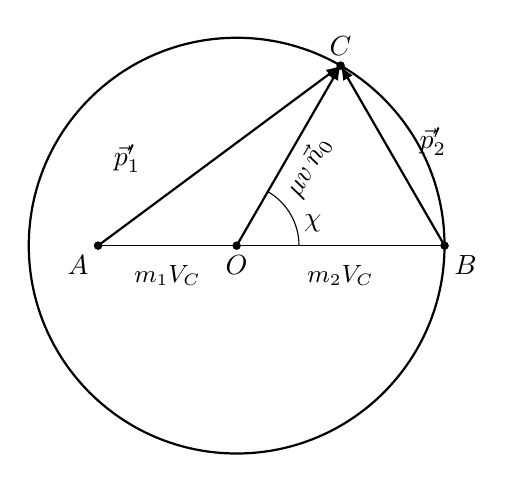
\begin{tikzpicture}[scale=2.2,>=latex]
  \coordinate (O) at (0,0);
  \coordinate (B) at (1.2,0);
  \coordinate (A) at (-0.8,0);
  \coordinate (C) at (60:1.2);
  \draw[thick] (O) circle (1.2);
  \draw (A)--(B);
  \draw[->,thick] (A)--(C);
  \draw[->,thick] (B)--(C);
  \draw[->,thick] (O)--(C) node[midway,sloped,below] {$\mu v\,\vec n_0$};
  \draw (0.36,0) arc (0:60:0.36);
  \node at (0.44,0.13) {$\chi$};
  \fill (A) circle (0.7pt); \fill (B) circle (0.7pt);
  \fill (O) circle (0.7pt); \fill (C) circle (0.7pt);
  \node[below left] at (A) {$A$};
  \node[below] at (O) {$O$};
  \node[below right] at (B) {$B$};
  \node[above] at (C) {$C$};
  \node[anchor=east] at (-0.50,0.50) {$\vec p_1'$};
  \node[anchor=west] at (1.00,0.60) {$\vec p_2'$};
  \node[below] at (-0.40,-0.06) {\small $m_1V_C$};
  \node[below] at (0.60,-0.06) {\small $m_2V_C$};
\end{tikzpicture}

{\small 图 1：动量圆。取 $m_1:m_2=2:3$（故 $A$ 在圆内）、$\chi=60^\circ$；圆心 $O$、半径 $|OB|=|OC|=\mu v_1$，$|AO|=\mu v_1\frac{m_1}{m_2}$。$A,O,B$ 三点共线、位置由碰前的量定死；$C$ 可以落在圆周上任意一处，落在哪由相互作用定。}
\end{center}

三点与半径的定义，逐条对上课件的记号（p9 右栏、p11 右栏）：

\par\vspace{2pt}
\noindent\begin{tabular}{@{}p{2.4cm}p{5.2cm}p{7.0cm}@{}}
\toprule
\thead{对象} & \thead{长度（矢量）} & \thead{来源}
\\
\midrule
$\overrightarrow{OC}$ & $\mu v$（半径）
& (2.1) 第一项。$|\overrightarrow{OC}|=\mu v$，方向 $\vec n_0$。\textbf{这就是"半径"的全部含义}：半径只能是 $\mu v$，因为 $|\vec n_0|=1$。
\\
$\overrightarrow{AO}$ & $\dfrac{m_1\,|\vec p_1+\vec p_2|}{m_1+m_2}=m_1V_C$
& (2.1) 第二项。p11 右栏手写把它算成 $\frac{m_1\cdot m_1v_1}{m_1+m_2}=\mu v_1\frac{m_1}{m_2}$（靶静止时）。
\\
$\overrightarrow{OB}$ & $\dfrac{m_2\,|\vec p_1+\vec p_2|}{m_1+m_2}=m_2V_C$
& 由 $\vec p_2'$ 的表达式。p11 右栏：「B 在圆周上，OB 是半径」——这句批注是在说 $|OB|=|OC|$。
\\
\bottomrule
\end{tabular}

靶静止时（$p_2=0$，即 p11 的「碰撞前 $p_2$ 为零；$v_2$ 为零」），三个长度都只剩一个数：
\[
|\overrightarrow{AB}|=p_1=m_1v_1,\qquad
|\overrightarrow{OB}|=\frac{m_2\,p_1}{m_1+m_2}=\mu v_1,\qquad
|\overrightarrow{AO}|=\frac{m_1\,p_1}{m_1+m_2}=\mu v_1\frac{m_1}{m_2}. \tag{2.2}
\]
检验：$|AO|+|OB|=\mu v_1\bigl(\frac{m_1}{m_2}+1\bigr)=\mu v_1\frac{m_1+m_2}{m_2}=m_1v_1=|AB|$，
且 $O$ 在 $A$、$B$ 之间。所以 $O$ \textbf{必在 $AB$ 上}，$B$ 必在圆周上，$A$ 在圆内还是圆外只看
\[
|AO|\gtrless|\overrightarrow{OB}|\iff \frac{m_1}{m_2}\gtrless 1\iff m_1\gtrless m_2 .
\]
这正是 p11 那两张圆图的区别：左图 $m_1<m_2$（$A$ 在圆内），右图 $m_1>m_2$（$A$ 在圆外）。
p9 那句 "When $\vec p_1$ and $\vec p_2$ are given, the radius of the circle and the points $A$ and $B$ are fixed, but the point $C$ can be located anywhere on the circle" 说的就是这件事——
它\textbf{不是}一条独立结论，而是 (2.2) 的直接读数。

\warnbox{\textbf{勘误（p4 的表述）}：p4 写「在质心坐标系下，没有总的动量!」。应说\textbf{总动量为零}。
每个粒子的动量当然不为零（p8 的 $\vec p_{10},\vec p_{20}$ 都在、p10 的图也全靠它们），为零的只是 $\vec p_{10}+\vec p_{20}$。
把"总动量为零"读成"没有动量"，后面 (1.4) 与整张圆图都没法建立。}

\subhdr{2.3　$\tan\th_1$ 的高度法（p11 先给结论，p12 才推）}

p11 把 $\tan\th_1=\frac{m_2\sin\chi}{m_1+m_2\cos\chi}$ 与 $\th_2=\frac{\pi-\chi}{2}$ 直接放进答案框（EXERCISE），
p12 才用"高度"推。p12 的推法只用一条竖线，是整章最省事的一段几何，但有三处没说明。补全：

\textbf{设置}：$D$ 是 $C$ 到直线 $AB$ 的垂足，$h=CD$。因 $O$ 是圆心、$|OC|=\mu v_1$ 是半径，
$\angle BOC=\chi$（这正是 $\chi$ 的定义：$\vec n_0$ 与 $\vec v$ 的夹角，而 $\vec v$ 沿 $AB$ 方向），于是

\[
h=|OC|\sin\angle BOC=\mu v_1\sin\chi,\qquad
OD=|OC|\cos\angle BOC=\mu v_1\cos\chi . \tag{2.3}
\]

\textbf{第一步}（p12 第一行）：在直角三角形 $ADC$ 中，$\tan\th_1=h/AD$，故 $h=AD\tan\th_1$。
\textbf{第二步}（p12 第二行"又 $AD=AO+OD$"）：把 (2.2) 的 $|AO|=\mu v_1\frac{m_1}{m_2}$ 与 (2.3) 的 $OD$ 相加：
\[
AD=\mu v_1\frac{m_1}{m_2}+\mu v_1\cos\chi=\mu v_1\Bigl(\frac{m_1}{m_2}+\cos\chi\Bigr). \tag{2.4}
\]
\textbf{第三步}：把 (2.3) 与 (2.4) 一起塞进 $h=AD\tan\th_1$，两边约掉 $\mu v_1$：
\[
\sin\chi=\Bigl(\frac{m_1}{m_2}+\cos\chi\Bigr)\tan\th_1
\ \Longrightarrow\
\tan\th_1=\frac{\sin\chi}{\frac{m_1}{m_2}+\cos\chi}=\frac{m_2\sin\chi}{m_1+m_2\cos\chi}. \tag{2.5}
\]
最后那步只是分子分母同乘 $m_2$。\hfill$\square$

\aside{(2.4) 里的 $AD=AO+OD$ 只在 $\chi<\pi/2$ 时自动成立。$\chi>\pi/2$ 时 $\cos\chi<0$，$D$ 跑到 $O$ 的另一侧，
此时 $AD=AO-|OD|$，而 (2.4) 因为 $\cos\chi$ 自带负号，\textbf{仍然是对的}——这就是为什么写 $\mu v_1\cos\chi$ 而不写 $\mu v_1|\cos\chi|$。
代数式不必分段，几何图形要分段。}

\warnbox{\textbf{勘误（p12 的记号）}：p12 第三行写 $h=\mu v_1\bigl(\frac{m_1}{m_2}+\cos\chi\bigr)\tan\th$，把下标 $1$ 丢了。
同一页第四、五行又写回 $\th_1$。本文统一写 $\th_1$。这类"下标掉一个"在这份课件里出现三次（p12、p22 的 $\mu v_\infty^2$ 与 $\mu v_\infty^4$、p25 的 $\mathrm L$ 与 $L$），都是排版而非物理。}

\subhdr{2.4　$\th_2$、最大散射角、方向的全部可能性（p11、p13）}

\textbf{（a）$\th_2=\frac{\pi-\chi}{2}$。}在三角形 $OBC$ 中，$|OB|=|OC|$（都是半径），故它是等腰三角形，
底角 $\angle OBC=\angle BCO=\frac{\pi-\angle BOC}{2}=\frac{\pi-\chi}{2}$。而 $\th_2$ 正是 $BC$（即 $\vec p_2'$）与 $AB$ 的夹角。
与质量无关，与 $U(r)$ 无关。

\textbf{（b）$\th_1+\th_2$ 与 $\frac\pi2$ 的大小。}这是 p13 底部那两行：
\[
\th_1+\th_2\;\begin{cases}>\dfrac{\pi}{2}, & m_1<m_2\\[2pt] <\dfrac{\pi}{2}, & m_1>m_2\end{cases}
\]
理由只有一条：把 $\chi=\pi-2\th_2$ 代进 (2.5)，得 $\tan\th_1=\frac{m_2\sin2\th_2}{m_1+m_2\cos2\th_2}$，而
$\th_1+\th_2-\frac\pi2$ 的符号与 $m_1-m_2$ 的符号相反。等号只在 $m_1=m_2$ 时成立（p16），此时两粒子恒成直角。

\textbf{（c）$\th_{\max}$（p13 右栏）。}$\sin\th_{\max}=\frac{OC}{OA}=\frac{m_2}{m_1}$，仅当 $m_1>m_2$。
几何理由：$\th_1$ 是 $AC$ 与 $AB$ 的夹角；$A$ 在圆外时，从 $A$ 能看到的最"斜"的方向就是圆的\textbf{切线}。
切线与圆心 $O$ 的连线垂直于切线，故在直角三角形 $AOC$ 中 $\sin\th_{\max}=\frac{|OC|}{|OA|}=\frac{m_2}{m_1}$。
$m_1<m_2$ 时 $A$ 在圆内，切线不存在，$AC$ 可以指向任何方向，故 p13 写 "any direction for $m_1$ after the collision is possible"。

\aside{取等号的时刻：切线对应 $\angle AOC=90^\circ$，即 $\angle BOC=\chi^{*}$ 满足 $\cos(\pi-\chi^*)=\frac{m_2}{m_1}$，
即 $\chi^*=\arccos\!\bigl(-\frac{m_2}{m_1}\bigr)$。课件只给 $\sin\th_{\max}$，没给这个 $\chi^*$；
做题时若问"最大角出现在哪个碰撞参数上"，要回到 §3 把 $\chi(\rho)$ 反解出来。}

\subhdr{2.5　$|v_1'|$ 与 $|v_2'|$：p13 的两个式子从哪来}

p13 在 EXERCISE 标签下给两式：
\[
v_1'=\frac{\sqrt{m_1^2+m_2^2+2m_1m_2\cos\chi}}{m_1+m_2}\,v,
\qquad
v_2'=\frac{2m_1\sin\frac\chi2}{m_1+m_2}\,v . \tag{2.6}
\]
第一式 p14--p15（两页手写）推了，第二式\textbf{没有任何一页推}。两个都补。

\textbf{（a）$v_1'$：余弦定理（p14--p15 的路子）。}三角形 $AOC$ 中 $\angle AOC=\pi-\chi$（$OA$ 与 $OB$ 反向、$\angle BOC=\chi$），故
\[
p_1'^2=AO^2+OC^2-2\,AO\cdot OC\cos(\pi-\chi) . \tag{2.7}
\]
p14 写到 (2.7) 就停了，p15 直接出现 $+2(\mu v_1\frac{m_1}{m_2})(\mu v_1)\cos\chi$ 的加号。中间那一步是
\[
\cos(\pi-\chi)=-\cos\chi\quad\Longrightarrow\quad -2\,AO\cdot OC\cos(\pi-\chi)=+2\,AO\cdot OC\cos\chi . \tag{2.8}
\]
代 $AO=\mu v_1\frac{m_1}{m_2}$、$OC=\mu v_1$：
\[
m_1^2v_1'^2=\Bigl(\mu v_1\frac{m_1}{m_2}\Bigr)^2+(\mu v_1)^2+2\Bigl(\mu v_1\frac{m_1}{m_2}\Bigr)(\mu v_1)\cos\chi .
\]
两边除 $m_1^2$，用 $\mu^2=\frac{(m_1m_2)^2}{(m_1+m_2)^2}$（p15 右侧红笔），得
\[
v_1'^2=\frac{v_1^2}{(m_1+m_2)^2}\Bigl(m_1^2+m_2^2+2m_1m_2\cos\chi\Bigr), \tag{2.9}
\]
开方取正根就是 (2.6) 第一式。\hfill$\square$

\textbf{（b）$v_2'$：课件缺的一步。}由 (1.4) 与伽利略变换，
\[
\vec v_2'=\vec v_{20}'+\vec V_C=-\frac{m_1v}{m_1+m_2}\vec n_0+\frac{m_1v}{m_1+m_2}\hat{\vec v}
=\frac{m_1v}{m_1+m_2}\bigl(\hat{\vec v}-\vec n_0\bigr),
\]
其中 $\hat{\vec v}$ 是 $\vec v$ 方向的单位矢量。于是
\[
v_2'^2=\Bigl(\frac{m_1v}{m_1+m_2}\Bigr)^2|\hat{\vec v}-\vec n_0|^2
=\Bigl(\frac{m_1v}{m_1+m_2}\Bigr)^2\cdot 2(1-\cos\chi)
=\Bigl(\frac{m_1v}{m_1+m_2}\Bigr)^2\cdot4\sin^2\frac\chi2 ,
\]
其中用了 $|\hat{\vec v}-\vec n_0|^2=2-2\cos\chi$（两个单位矢量之差的长度公式）。开方得 (2.6) 第二式。\hfill$\square$

\aside{两个因子的分工不同，别混：（2.6）第一式的 $2m_1m_2\cos\chi$ 来自\textbf{余弦定理的角度项}；第二式的 $4\sin^2\frac\chi2$ 来自\textbf{半角公式} $1-\cos\chi=2\sin^2\frac\chi2$，再乘平方里的 $2$ 得 $4$。
前者是几何，后者是三角恒等式。}

\subhdr{2.6　等质量：碰后恒成直角（p16）}

$m_1=m_2\equiv m$ 时，(2.2) 给出 $|AO|=|OB|=\mu v_1=\frac{m}{2}v_1$，故 $O$ 是 $AB$ 的中点、$A$、$B$ 都在圆上。于是：

\begin{itemize}
\item 三角形 $OBC$ 仍是等腰，$\th_2=\frac{\pi-\chi}{2}$；
\item 三角形 $AOC$ 中 $|AO|=|OC|$（都等于半径），也是等腰，故 $\th_1=\angle OAC=\frac{\pi-\angle AOC}{2}=\frac{\pi-(\pi-\chi)}{2}=\frac\chi2$；
\item 于是 $\th_1+\th_2=\frac\chi2+\frac{\pi-\chi}{2}=\frac\pi2$。
\end{itemize}
速度则代 $\chi=2\th_1$ 进 (2.6)：$v_1'=v\cos\frac\chi2$、$v_2'=v\sin\frac\chi2$，且 $v_1'^2+v_2'^2=v^2$。
p16 的 "After the collision the particles move at \textbf{right angles} to each other!" 与 "$A+B=\frac\pi2$" 就是这一段。
p16 右栏那张手写照片则是 (2.5) 在 $m_1=m_2$ 时的化简：
$\tan\th_1=\frac{\sin\chi}{1+\cos\chi}=\frac{2\sin\frac\chi2\cos\frac\chi2}{1+2\cos^2\frac\chi2-1}=\tan\frac\chi2$。

\subhdr{2.7　完整算例：$m_1=2$、$m_2=3$、$\chi=60^\circ$}

把 §2 的每一式都过一遍数，取 $v_1=1$（单位任取）、靶静止。

\begin{enumerate}[label=(\arabic*)]
\item \textbf{圆图}：$|AB|=p_1=2$；$|OB|=\mu v_1=\frac{6}{5}\cdot1=1.2$；$|AO|=1.2\cdot\frac23=0.8$。检验 $0.8+1.2=2=|AB|$，且 $0.8<1.2$ 故 $A$ 在圆内（$m_1<m_2$）。
\item \textbf{角度}：$\tan\th_1=\frac{3\sin60^\circ}{2+3\cos60^\circ}=\frac{2.5981}{3.5}=0.74231$，$\th_1=36.587^\circ$；$\th_2=\frac{180^\circ-60^\circ}{2}=60^\circ$。
$\th_1+\th_2=96.587^\circ>\frac\pi2$，与 $m_1<m_2$ 相符（§2.4b）。
\item \textbf{速率}：$v_1'=\frac{\sqrt{4+9+2\cdot6\cdot0.5}}{5}=\frac{\sqrt{19}}{5}=0.87178$；$v_2'=\frac{2\cdot2\cdot\sin30^\circ}{5}=0.4$。
\item \textbf{自检（能量）}：$\frac12 m_1v_1'^2=\frac{19}{25}=0.76$，$\frac12m_2v_2'^2=\frac{3}{2}\cdot0.16=0.24$，和 $=1.00=\frac12m_1v_1^2$。
\item \textbf{自检（动量）}：水平分量 $m_1v_1'\cos\th_1+m_2v_2'\cos\th_2=2(0.87178)(0.80304)+3(0.4)(0.5)=1.4000+0.6000=2.00=m_1v_1$；
竖直分量 $2(0.87178)(0.59588)-3(0.4)(0.86603)=1.0391-1.0392\approx0$。
\end{enumerate}

第 (4)(5) 两问是这道小算例的全部意义：\textbf{几何法算出来的角度与速率，必须回到两条守恒律去验}。
如果哪一步算错，通常错在第 (5) 的竖直分量上——因为 $\th_2$ 的方向（向上还是向下）在圆图上左右对称，写公式时最容易漏负号。

%=============================================================
\hdr{§3}{主线 B：从轨道到截面（p17--p21）}

\subhdr{3.1　有心力轨道的对称性：$\chi=|\pi-2\varphi_0|$}

p17 的两句英文是这一节的骨架：

\begin{quote}
"The \textbf{path} of a particle in a central field is \textbf{symmetric} in respect to a line connecting the field center with the nearest point of the orbit."
\end{quote}
\begin{quote}
$r_{\min}$ "is the zero of the radicand"
\end{quote}
配上同页两个式子（p17 中部与右栏）：
\[
\chi=|\pi-2\varphi_0|,\qquad
\varphi_0=\int_{r_{\min}}^{\infty}\frac{\frac{L}{r^2}\dd r}{\sqrt{2\mu\bigl(E-U(r)\bigr)-\frac{L^2}{r^2}}} .
\]

"对称"这一步课件没证。理由是\textbf{时间反演}：有心力场里 $m\ddot{\vec r}=F(r)\hat{\vec r}$，
把 $t\to-t$、$\dot{\vec r}\to-\dot{\vec r}$ 之后方程不变，所以"从 $r_{\min}$ 冲出去"的轨道倒着走就是"冲进来"的轨道。
于是\textbf{进来与出去两段关于最近点连线镜像}：进来扫过 $\varphi_0$，出去也扫过 $\varphi_0$，全程 $\Delta\varphi=2\varphi_0$。

\aside{p17 右栏还写了 $\Delta\phi=2\int\dd r\,\frac{L}{r^2}\bigl[2\mu(E-U)-\frac{L^2}{r^2}\bigr]^{-1/2}$——这就是 $2\varphi_0$。
批注「被开方数」指的就是根号里的那个式子：它在 $r=r_{\min}$ 处为零，这正是 $r_{\min}$ 的定义。}

有了 $\Delta\varphi=2\varphi_0$，偏转角就是把"本来是直线"补回来：
若无相互作用，粒子沿直线走，$\Delta\varphi=0$；实际转了 $2\varphi_0$，所以偏离原方向 $|\pi-2\varphi_0|$。
取绝对值是因为 $\varphi_0$ 可以超过 $\pi/2$（强偏转、甚至绕进中心），此时 $\pi-2\varphi_0<0$，偏转角取正值 $2\varphi_0-\pi$。

\warnbox{\textbf{(3.1) 的适用条件（课件没写）}：
（i）$r_{\min}$ 必须是\textbf{被开方数的零点}。若被开方数处处为正（例如 $L$ 很大、能量很高、势又弱），
粒子根本进不到 $r_{\min}$，全程近似直线，$\varphi_0\to\pi/2$、$\chi\to0$，这是"擦边而过"的极限；
若被开方数在某个 $r$ 处为零但之后变负（吸引势太强），粒子\textbf{落进中心}（capture），$r_{\min}$ 之外没有轨道，
此时 (3.1) 不适用、$\chi$ 无定义——截面上会出现一个"吸收"的洞。
（ii）$U(r)\to0$（$r\to\infty$）是"$E$ 就是无穷远动能"的前提，否则 $E$ 与 $v_\infty$ 的关系要改。}

\subhdr{3.2　换参数：$(E,L)\to(v_\infty,\rho)$（p18）}

p18 的中文批注说「转换一下思路，我们从两个守恒量出发 能量和角动量 变换一下运动积分」，然后给
\[
E=\frac{\mu v_\infty^2}{2},\qquad L=\mu\rho v_\infty . \tag{3.2}
\]
两条都要交代清楚：

\textbf{$E=\mu v_\infty^2/2$}：无穷远处 $U=0$、速率 $v_\infty$，故相对运动的能量就是 $\frac{\mu v_\infty^2}{2}$。
这正是 (1.1) 里"能量守恒"那一条在 $t\to-\infty$ 的取值。

\textbf{$L=\mu\rho v_\infty$}：角动量关于力心守恒（有心力 $\Rightarrow$ 力矩为零），
在无穷远处取"入射直线到力心的垂距"$\rho$ 与速率 $v_\infty$，角动量就是 $\mu\rho v_\infty$。

\aside{角动量守恒的前提：$U=U(r)$ 只依赖 $r$，力矩 $\vec r\times F(r)\hat r=0$（Topic 5 有心力一节）。
所以 $L$ 在整个过程中是常数，可以用\textbf{任意一点}算——本文一律用无穷远处算，因为那里最省事。
代入本题：$\rho$ 是碰撞参数（瞄准距离），不是密度。}

把 (3.2) 代进 $\varphi_0$ 的求积，就消掉了 $L$ 与 $\sqrt{2\mu E}$：
\[
\varphi_0=\int_{r_{\min}}^{\infty}\frac{\rho\,\dd r/r^2}{\sqrt{1-\dfrac{\rho^2}{r^2}-\dfrac{2U(r)}{\mu v_\infty^2}}} . \tag{3.3}
\]
（推导：根号里提出 $2\mu E=2\mu\cdot\frac{\mu v_\infty^2}{2}=\mu^2v_\infty^2$，被积函数分子提出 $\frac{L}{\sqrt{2\mu E}}=\frac{\mu\rho v_\infty}{\mu v_\infty}=\rho$。）
p18 下方那两式就是 (3.3) 与它的原始形式并排。于是 p18 最后那个方框
\[
\chi=\chi(\rho)
\]
的意思是：\textbf{$\varphi_0$ 只是 $\rho$ 的函数，所以 $\chi$ 也只是 $\rho$ 的函数}。整条散射问题的因果链到这里才成形：
给 $U(r)$ $\to$ (3.3) 得 $\varphi_0(\rho)$ $\to$ $\chi(\rho)$ $\to$ 截面。

\subhdr{3.3　有效截面 $\dd\sigma$：定义、几何、换变量}

p19 与 p21 各给了一遍同一件事，p21 那一遍多了量纲和一个"为什么"。按逻辑顺序重排（课件是三块并排，顺序是乱的）：

\callout{\textbf{定义 1（有效截面，p19/p21）}
设束流中单位时间穿过单位面积的入射粒子数为 $n$（粒子数密度 $\times$ 速率），
单位时间内在 $\chi$ 与 $\chi+\dd\chi$ 之间被散开的粒子数为 $\dd N$。定义
\[
\dd\sigma\equiv\frac{\dd N}{n} . \tag{3.4}
\]
量纲：$[\dd N]=\mathrm{s^{-1}}$、$[n]=\mathrm{m^{-2}s^{-1}}$，故 $[\dd\sigma]=\mathrm{m^2}$——它是一个\textbf{面积}。
p21 右栏这一行算得没错：「$\frac{\dd N}{n}=\frac{1/s}{1/(m^2s)}=m^2$」。}

\textbf{为什么不用 $\dd N$ 而用 $\dd\sigma$}：p21 左栏自己回答了——
"$\dd N$ itself is not suitable for describing the scattering since it is proportional to the density of the incident beam."
同一块靶、同样的相互作用，把束流调密一倍，$\dd N$ 就翻倍；但"靶有多大的有效面积"不该随束流变。
除掉 $n$ 之后剩下的才是靶的性质。这就是"有效"两个字。

\textbf{从定义到 $2\pi\rho\dd\rho$（p19/p21 的几何）}：碰撞参数落在 $(\rho,\rho+\dd\rho)$ 里的入射粒子，
打在一个半径为 $\rho$、宽 $\dd\rho$ 的圆环上，面积
\[
\dd\sigma=2\pi\rho\,\dd\rho . \tag{3.5}
\]
这一步之所以成立，靠的是"束流均匀"（p19："incident with the uniform velocity $v_\infty$"）——
均匀意味着"面积正比于粒子数"，(3.4) 里的 $n$ 才可以提到外面。

\textbf{换变量：$\rho\to\chi$}。由 §3.2，$\chi=\chi(\rho)$ 是确定的关系，所以同一个 $\dd N$ 可以用 $\dd\chi$ 记账。
把 (3.5) 里的 $\dd\rho$ 用 $\dd\chi$ 表示，注意\textbf{$\chi$ 随 $\rho$ 增大而减小}（远处掠过偏转小、正撞偏转大），
所以 $\dd\rho/\dd\chi<0$，取绝对值：
\[
\dd\sigma=2\pi\rho(\chi)\Bigl|\frac{\dd\rho}{\dd\chi}\Bigr|\dd\chi . \tag{3.6}
\]
p31 右栏对此有一句说明："Here we use the modulus of the derivative ... Since the derivative may be (usually) negative"。
"usually"用得很准：只有 $U$ 单调时它才总是负的。

\warnbox{\textbf{适用条件（p21 的断言要打折扣）}：p21 右栏末行说 "the relation between $\chi$ and $\rho$ is \textbf{one-to-one}"。
这句话只在 $U(r)$ 单调（且无捕获）时成立。反例：有效势 $U_{\rm eff}=U+L^2/2\mu r^2$ 有极小值时，$\chi(\rho)$ 会多值——
同一个 $\chi$ 对应几个 $\rho$，此时 (3.6) 要\textbf{对所有分支求和}：
$\dd\sigma=\sum_i 2\pi\rho_i|\dd\rho_i/\dd\chi|\dd\chi$。
课件没给这个求和，凡遇到"轨道回旋"的势都必须自己补。
\textbf{[教材补充]}：Landau《Mechanics》§18 在给出同一公式后明确说，若 $\chi(\rho)$ 非单值，须对 $\rho$ 的各支求和。}

\subhdr{3.4　立体角与 $\dd\sigma/\dd\Omega$}

p20 用一整页讲立体角，中文批注只有两个词：「立体角」「$\dd\Omega=\dd A/r^2$」；正文给
\[
\dd\Omega=\sin\th\,\dd\th\,\dd\phi,\qquad [\Omega]=\text{steradian},\qquad \text{总立体角}=4\pi . \tag{3.7}
\]
三条互相独立，逐条落地：

\textbf{（i）$\dd\Omega=\dd A/r^2$ 与 (3.7) 是同一件事。}在半径 $r$ 的球面上，一块"经纬度分别为 $\dd\th,\dd\phi$"的小面元
边长是 $r\dd\th$ 与 $r\sin\th\,\dd\phi$，故 $\dd A=r^2\sin\th\,\dd\th\,\dd\phi$，除以 $r^2$ 就是 (3.7)。
所以中文批注与公式不矛盾，前者是定义、后者是球坐标下的读数。

\textbf{（ii）总立体角 $4\pi$ 是"约定"，不是"数学"。}\ $\int_0^{\pi}\!\sin\th\dd\th\int_0^{2\pi}\!\dd\phi=2\times2\pi=4\pi$。
这里的 $4\pi$ 来自"球面度"这个单位制约定（把整个球面对球心的张角定为 $4\pi$ 球面度），
与 (3.7) 里的 $\sin\th$ 分工不同：$\sin\th$ 是球面几何，$4\pi$ 是归一化约定。

\textbf{（iii）绕轴旋转对称时 $\dd\Omega=2\pi\sin\chi\dd\chi$。}有心力问题里 $\chi$ 就是极角、$\phi$ 是绕束流的方位角，
被积函数与 $\phi$ 无关，$\int_0^{2\pi}\dd\phi=2\pi$，于是
\[
\dd\Omega=2\pi\sin\chi\,\dd\chi . \tag{3.8}
\]
p19 与 p31 都写着这一行（p31 是手写：「$\dd\Omega=\sin\th\dd\th\dd\phi\to2\pi\sin\chi\dd\chi$」）。

\textbf{（iv）单位立体角的截面。}把 (3.6) 除 (3.8)：
\[
\frac{\dd\sigma}{\dd\Omega}
=\frac{2\pi\rho(\chi)\bigl|\frac{\dd\rho}{\dd\chi}\bigr|\dd\chi}{2\pi\sin\chi\,\dd\chi}
=\frac{\rho(\chi)}{\sin\chi}\Bigl|\frac{\dd\rho}{\dd\chi}\Bigr| . \tag{3.9}
\]
(3.9) 就是 p19 与 p31 那个框里的公式。它是整章最有用的一行：
\textbf{只要知道 $\rho(\chi)$，(3.9) 一步给出实验上真正测的量}。

\aside{(3.9) 的两个因子来源不同：分母的 $\sin\chi$ 来自立体角的球面几何 (3.8)；
$|\dd\rho/\dd\chi|$ 来自"把 $\rho$ 的账换成 $\chi$ 的账"时的雅可比 (3.6)。
前者是几何，后者是换元。两者都不可省——省掉 $\sin\chi$ 就得到 $\dd\sigma/\dd\chi$（对 $\chi$ 的微分截面），
省掉 $|\dd\rho/\dd\chi|$ 就得到"对 $\rho$ 的微分截面"，都不是探测器读到的那个量。}

%=============================================================
\hdr{§4}{两条线怎么接：C 系截面 $\to$ 实验室系截面（p20、p29、p30、p11）}

\subhdr{4.1　为什么可以直接换}

p20 下半页只有两句：

\begin{quote}
"In case of scattering of particles not by a fixed center of force, but by the other particles which are initially at rest, the expression above gives DCS in the \textbf{C-frame}. In order to switch to the laboratory frame, one should use the transformation expressions:"\quad 配 $\tan\th_1=\frac{m_2\sin\chi}{m_1+m_2\cos\chi}$,\ $\th_2=\frac{\pi-\chi}{2}$
\end{quote}

这里有一个\textbf{拼接缺口}，值得单列：$\tan\th_1$ 与 $\th_2$ 这两式，本来是在 p11 的"动量圆"上、针对\textbf{靶静止}的碰撞推出来的（§2.3、§2.4），
而 p20 要换的却是一般的 $U(r)$ 散射。凭什么能搬过来？

理由是：这两式\textbf{只用到两条与 $U(r)$ 无关的事实}——
（i）C 系里碰后两粒子动量反向等大（定理 1），故 $|OB|=|OC|$、三角形 $OBC$ 等腰；
（ii）实验室系 = C 系 + 整体平移 $\vec V_C$（伽利略）。
所以任何"在 C 系里出射方向为 $\vec n_0$、速率为 $\mu v/m_i$"的过程，都能用同一张圆图换算，\textbf{不管 $\chi$ 是怎么来的}。
换句话说：$\chi$ 的数值由 $U(r)$ 定（§3.2），$\chi\to\th_1,\th_2$ 的换算由质量比定（§2）。两者互不干涉，这正是可以分两步做的原因。

\subhdr{4.2　$\chi=\pi-2\th_2$ 与 $\dd\sigma_2$（p29 第一式）}

p29 第一行："Switching to the L-frame, for particles which are initially at rest we obtain: $\chi=\pi-2\th_2$"。
这不过是 §2.4(a) 的 $\th_2=\frac{\pi-\chi}{2}$ 反过来写，对\textbf{靶粒子}成立。

把 $\dd\sigma$ 从 $(\chi,\dd\chi)$ 换到 $(\th_2,\dd\th_2)$，要换三个东西：
\begin{itemize}
\item $\dd\chi\to\dd\th_2$：$\chi=\pi-2\th_2\Rightarrow|\dd\chi|=2\dd\th_2$；
\item $\sin\frac\chi2\to\cos\th_2$：$\sin\frac{\pi-2\th_2}{2}=\sin\bigl(\frac\pi2-\th_2\bigr)=\cos\th_2$；
\item $\sin\chi\,\dd\chi\to\sin\th_2\,\dd\th_2$：$\sin\chi=\sin(2\th_2)=2\sin\th_2\cos\th_2$，再乘 $|\dd\chi|=2\dd\th_2$，共 $4\sin\th_2\cos\th_2\,\dd\th_2$。
\end{itemize}

其中第三组的意思是：$\dd\Omega_C=4\cos\th_2\,\dd\Omega_2$（$2\pi$ 已约掉）。合并起来：
\[
\dd\sigma_2=\Bigl(\frac{\alpha}{2\mu v_\infty^2}\Bigr)^2\frac{\dd\Omega_C}{\sin^4\frac\chi2}
=\Bigl(\frac{\alpha}{2\mu v_\infty^2}\Bigr)^2\frac{4\cos\th_2\,\dd\Omega_2}{\cos^4\th_2}
=\Bigl(\frac{\alpha}{\mu v_\infty^2}\Bigr)^2\frac{\dd\Omega_2}{\cos^3\th_2}. \tag{4.1}
\]
写成 p29 的样子（把 $\dd\Omega_2=2\pi\sin\th_2\dd\th_2$ 拆开）就是
\[
\dd\sigma_2=2\pi\Bigl(\frac{\alpha}{\mu v_\infty^2}\Bigr)^2\frac{\sin\th_2}{\cos^3\th_2}\dd\th_2 . \tag{4.2}
\]
(4.2) 与 p29 第一式的左半逐字相同。

\warnbox{\textbf{勘误（p29 第一式的右半）}：p29 写
$\dd\sigma_2=\bigl(\frac{\alpha}{\mu v_\infty^2}\bigr)^2\frac{\dd\Omega_2}{(\cos\th_2)^4}$，分母是 \textbf{四次}。
但同一式的左半是 $\frac{\sin\th_2}{(\cos\th_2)^3}\dd\th_2$，而 $2\pi\sin\th_2\dd\th_2=\dd\Omega_2$，
故右半只能是 $\frac{\dd\Omega_2}{(\cos\th_2)^3}$。三方对账（(4.1) 的独立推导、p29 左半、p29 末行的全同粒子求和式）都指向\textbf{三次}。
本文用三次。这个指数很要紧：它决定"靶粒子谱在 $\th_2\to\pi/2$ 处发散"的强弱。}

\subhdr{4.3　等质量时 $\dd\Omega_C=4\cos\th_1\,\dd\Omega_1$（p30）}

p30 把 p29 的换算在 $m_1=m_2$ 下重做了一遍，写成一行三个等号：
\[
\dd\Omega=2\pi\sin2\th_1\,\dd(2\th_1)=8\pi\sin\th_1\cos\th_1\,\dd\th_1=4\cos\th_1\,\dd\Omega_1 .
\]
三个等号各用了什么：

\begin{enumerate}[label=(\arabic*)]
\item 第一个等号：$\chi=2\th_1$（§2.6），所以 $\sin\chi\to\sin2\th_1$、$\dd\chi\to\dd(2\th_1)=2\dd\th_1$。这一步只做了代换，还没整理。
\item 第二个等号：用 $\sin2\th_1=2\sin\th_1\cos\th_1$ 与 $\dd(2\th_1)=2\dd\th_1$，系数 $2\pi\times2\times2=8\pi$。
\item 第三个等号：把 $8\pi\sin\th_1\cos\th_1\dd\th_1$ 里"属于 $\dd\Omega_1$ 的部分"认出来——
$\dd\Omega_1=2\pi\sin\th_1\dd\th_1$，剩下 $4\cos\th_1$。所以 $8\pi\cdots=4\cos\th_1\cdot(2\pi\sin\th_1\dd\th_1)$。
\end{enumerate}
于是 $\dd\sigma_1=\bigl(\frac{\alpha}{2\mu v_\infty^2}\bigr)^2\frac{4\cos\th_1\dd\Omega_1}{\sin^4\th_1}$，
再用 $2\mu v_\infty^2=m_1v_\infty^2=2E_1$（等质量时 $\mu=m_1/2$）与 $\bigl(\frac{\alpha}{2E_1}\bigr)^2\cdot4=\bigl(\frac{\alpha}{E_1}\bigr)^2$，得 p29 的 2) 式：
\[
\dd\sigma_1=\Bigl(\frac{\alpha}{E_1}\Bigr)^2\frac{\cos\th_1\,\dd\Omega_1}{\sin^4\th_1}. \tag{4.3}
\]

\subhdr{4.4　两个极限（p29 的 1) 与 2)）}

\textbf{极限 1：$m_2\gg m_1$。}此时 $\mu=\frac{m_1m_2}{m_1+m_2}\to m_1$，$E\to E_1$；
几何上 $|AO|\to0$（$A$ 塌到 $O$ 上），$AC$ 与 $OC$ 几乎重合，故 $\th_1\approx\chi$。代入 (3.9) 型公式：
\[
\dd\sigma_1=\Bigl(\frac{\alpha}{2\mu v_\infty^2}\Bigr)^2\frac{\dd\Omega_1}{\sin^4\frac{\th_1}{2}}
\;\xrightarrow{m_2\gg m_1}\;
\Bigl(\frac{\alpha}{4E_1}\Bigr)^2\frac{\dd\Omega_1}{\sin^4\frac{\th_1}{2}} . \tag{4.4}
\]
（用了 $\frac{\alpha}{2\mu v_\infty^2}=\frac{\alpha}{4E}\to\frac{\alpha}{4E_1}$。）这就是"重靶"情形：靶几乎不动，实验室系就是质心系。

\textbf{极限 2：$m_2=m_1$。}$\mu=m_1/2$、$E=E_1/2$，$\chi\approx2\th_1$，结果就是 (4.3)。
两个极限的差别只在两处：质量因子（$\mu$ 换成 $m_1$ 还是 $m_1/2$）与角度因子（$\chi$ 换成 $\th_1$ 还是 $2\th_1$）。

\subhdr{4.5　全同粒子：两项之和（p29 末行）}

p29 最后一行："totally identical particles can not be distinguished"，配
\[
\dd\sigma=\Bigl(\frac{\alpha}{E_1}\Bigr)^2\Bigl(\frac{1}{\sin^4\th}+\frac{1}{\cos^4\th}\Bigr)\cos\th\,\dd\Omega . \tag{4.5}
\]
为什么是两项之和：探测器摆在实验室系角度 $\th$ 处，它数到的粒子可能是
（i）\textbf{入射粒子}被偏转 $\th$——此时 $\chi=2\th$，贡献 (4.3)，即 $\frac{\cos\th}{\sin^4\th}$ 项；
（ii）\textbf{靶粒子}被反冲 $\th$——此时 $\th_2=\th$，$\chi=\pi-2\th$，$\sin\frac\chi2=\cos\th$，贡献 (4.1) 的 $\frac{\cos\th}{\cos^4\th}=\frac{1}{\cos^3\th}$ 项。
两个粒子不可分辨，故把两个贡献\textbf{相加}（不是干涉，是计数）。

核对 (ii) 与 (4.5) 第二项：$\bigl(\frac{\alpha}{E_1}\bigr)^2\frac{\cos\th}{\cos^4\th}=\bigl(\frac{\alpha}{E_1}\bigr)^2\frac{1}{\cos^3\th}$，
而 §4.2 得 $\dd\sigma_2/\dd\Omega_2=\bigl(\frac{\alpha}{\mu v_\infty^2}\bigr)^2\frac{1}{\cos^3\th_2}=\bigl(\frac{\alpha}{E_1}\bigr)^2\frac1{\cos^3\th_2}$（等质量时 $\mu v_\infty^2=E_1$），一致。
\textbf{[教材补充]}：Landau《Mechanics》§18 末段讨论同一问题，做法与理由都是"把两个粒子在实验室系中的截面相加"（不可分辨 $\Rightarrow$ 计数叠加）。

\aside{(4.5) 在 $\th\to\frac\pi2$ 处两项都发散（正向项的 $\sin^{-4}$ 与反向项的 $\cos^{-4}$ 各管一头），
这正是"等质量碰撞在 $90^\circ$ 附近计数最多"的定量形式；$\th=\frac\pi4$ 处两项相等，是最"对称"的观测角。}

%=============================================================
\hdr{§5}{主例题全程演算：卢瑟福公式的四步链（p22--p26、p31、p34）}

这是这份课件里唯一一道"从 $U(r)$ 一路推到 $\dd\sigma/\dd\Omega$"的完整题（p22 标 EXERCISE）。
课件用了五页正文加两张手写页，但每一步都跳。本节按四个步骤重走一遍，每步都补上被跳掉的代数。

\subhdr{5.1　第一步：把 $\varphi_0$ 积出来（p23--p24）}

\textbf{题}：$U(r)=\alpha/r$（$\alpha>0$，排斥），$E$、$\rho$ 给定，求 $\varphi_0$。

代入 (3.3)：
\[
\varphi_0=\int_{r_{\min}}^{\infty}\frac{\rho\,\dd r/r^{2}}{\sqrt{1-\dfrac{\rho^{2}}{r^{2}}-\dfrac{2\alpha}{\mu v_\infty^{2}}\cdot\dfrac{1}{r}}} . \tag{5.1}
\]

\textbf{换元 $u=1/r$}。这一步是整道题的关键，课件完全没写（p23 一上来就是 $\phi=\arccos(\cdots)$ 的开普勒结果）。换元账要算清：
\[
u=\frac1r,\qquad \dd u=-\frac{\dd r}{r^{2}},\qquad r=r_{\min}\to u=\frac{1}{r_{\min}},\qquad r=\infty\to u=0 .
\]
注意 $\dd r/r^2=-\dd u$，上下限方向相反，两个负号抵消：
\[
\varphi_0=\int_{0}^{1/r_{\min}}\frac{\rho\,\dd u}{\sqrt{1-\rho^{2}u^{2}-\beta u}},
\qquad \beta\equiv\frac{2\alpha}{\mu v_\infty^{2}} . \tag{5.2}
\]

\textbf{配方}。被开方数对 $u$ 是二次式，配方：
\[
1-\rho^{2}u^{2}-\beta u
=\underbrace{1+\frac{\beta^{2}}{4\rho^{2}}}_{\textstyle A^{2}}-\rho^{2}\Bigl(u+\frac{\beta}{2\rho^{2}}\Bigr)^{2},
\qquad A^{2}\equiv1+\frac{\beta^{2}}{4\rho^{2}}=1+\frac{\alpha^{2}}{\mu^{2}v_\infty^{4}\rho^{2}} . \tag{5.3}
\]
（末一等号用了 $\beta^2/4\rho^2=\frac{4\alpha^2}{\mu^2v_\infty^4}\big/4\rho^2$。）这个 $A$ 就是 p24 里根号下的那个 $1+\bigl(\frac{\alpha}{\mu v_\infty^2\rho}\bigr)^2$。

\textbf{再换元消掉配方}。令 $\rho\bigl(u+\frac{\beta}{2\rho^{2}}\bigr)=A\sin w$，则 $\rho\,\dd u=A\cos w\,\dd w$，被开方数 $=A^2\cos^2w$，于是
\[
\varphi_0=\int\frac{A\cos w\,\dd w}{A\cos w}=\int\dd w=w\Big|_{\text{下}}^{\text{上}} .
\]
上下限怎么定？这是全题最容易被蒙过去的一处，而课件 p17 已经给了钥匙——「$r_{\min}$ is the zero of the radicand」：

\begin{itemize}
\item \textbf{上限} $u=1/r_{\min}$ 处被开方数为零（$r_{\min}$ 的定义），故 $A\sin w_{\text{上}}=A$，即 $w_{\text{上}}=\frac\pi2$；
\item \textbf{下限} $u=0$ 处 $\rho\bigl(0+\frac{\beta}{2\rho^{2}}\bigr)=\frac{\beta}{2\rho}=\frac{\alpha}{\mu v_\infty^2\rho}$，故
$A\sin w_{\text{下}}=\frac{\alpha}{\mu v_\infty^2\rho}$，即 $\sin w_{\text{下}}=\frac{\alpha/(\mu v_\infty^2\rho)}{A}$。
\end{itemize}
于是 $\varphi_0=\frac\pi2-w_{\text{下}}$，而 $\sin w_{\text{下}}=\cos\varphi_0$，所以
\[
\varphi_0=\arccos\frac{\dfrac{\alpha}{\mu v_\infty^{2}\rho}}{\sqrt{1+\Bigl(\dfrac{\alpha}{\mu v_\infty^{2}\rho}\Bigr)^{2}}} . \tag{5.4}
\]
(5.4) 与 p22/p24 的方框逐字相同。\hfill$\square$

\aside{(5.4) 只依赖一个无量纲组合 $\dfrac{\alpha}{\mu v_\infty^2\rho}=\dfrac{\alpha}{2E\rho}$，
即"碰撞参数处的库仑势能"与"入射动能 $\times 2$"之比。$\rho\to\infty$ 时它 $\to0$，$\varphi_0\to\frac\pi2$（直线掠过）；$\rho\to0$ 时它 $\to\infty$，$\varphi_0\to0$（正撞，直穿）。}

\subhdr{5.2　第二步：从 $\varphi_0$ 到 $\rho(\chi)$（p25 右栏）}

只用两条：$\chi=\pi-2\varphi_0\Rightarrow\varphi_0=\frac\pi2-\frac\chi2$，以及恒等式 $\tan^2\varphi_0=\frac{1-\cos^2\varphi_0}{\cos^2\varphi_0}$。

\textbf{（a）$\cos\varphi_0$ 与 $\tan^2\varphi_0$}。记 $X\equiv\frac{\alpha}{\mu v_\infty^2\rho}$，则 (5.4) 是 $\cos\varphi_0=\frac{X}{\sqrt{1+X^2}}$，于是
\[
\sin^2\varphi_0=1-\frac{X^2}{1+X^2}=\frac{1}{1+X^2},
\qquad
\tan^2\varphi_0=\frac{\sin^2\varphi_0}{\cos^2\varphi_0}=\frac{1}{X^2} . \tag{5.5}
\]
p25 右栏写的是 $\tan^2\phi_0=\cot^2\frac\chi2=\dfrac{1}{\bigl(\frac{\alpha}{\mu v_\infty^2\rho}\bigr)^2}$，与 (5.5) 一致
（$\varphi_0=\frac\pi2-\frac\chi2\Rightarrow\tan\varphi_0=\cot\frac\chi2$）。

\textbf{（b）解出 $\rho^2$}。由 (5.5)：$\cot^2\frac\chi2=\frac{1}{X^2}=\bigl(\frac{\mu v_\infty^2\rho}{\alpha}\bigr)^2$，两边乘 $\frac{\alpha^2}{\mu^2v_\infty^4}$：
\[
\rho^{2}=\frac{\alpha^{2}}{\mu^{2}v_\infty^{4}}\cot^{2}\frac\chi2
\qquad\Longleftrightarrow\qquad
\rho=\frac{\alpha}{\mu v_\infty^{2}}\cot\frac\chi2=\frac{\alpha}{2E}\cot\frac\chi2=k\cot\frac\chi2 . \tag{5.6}
\]
（末一等号用 $\mu v_\infty^2=2E$ 与 $k\equiv\alpha/(2E)$。）(5.6) 与 p22、p25 的方框一致。

\subhdr{5.3　第三步：$\rho\,\dd\rho/\dd\chi$（p25、p26、p31）}

\textbf{方法一（p26/p31 的路子：先乘 $\rho$，再求导）}。由 (5.6)，
\[
\frac{\dd\rho}{\dd\chi}=k\cdot\Bigl(-\frac{1}{2\sin^{2}\frac\chi2}\Bigr)=-\frac{k}{2\sin^{2}\frac\chi2},
\qquad
\Bigl|\frac{\dd\rho}{\dd\chi}\Bigr|=\frac{k}{2\sin^{2}\frac\chi2} . \tag{5.7}
\]
（这里用了 $\frac{\dd}{\dd\chi}\cot\frac\chi2=-\frac{1}{2}\csc^2\frac\chi2$，p25 下方就贴着 $\cot$ 的导数表 $y'=-\frac{1}{\sin^2x}$。）
于是
\[
2\pi\rho\Bigl|\frac{\dd\rho}{\dd\chi}\Bigr|\dd\chi
=2\pi\cdot k\cot\frac\chi2\cdot\frac{k}{2\sin^2\frac\chi2}\,\dd\chi
=\pi k^{2}\frac{\cos\frac\chi2}{\sin^{3}\frac\chi2}\,\dd\chi . \tag{5.8}
\]
（用了 $\cot\frac\chi2/\sin^2\frac\chi2=\cos\frac\chi2/\sin^3\frac\chi2$。）这就是 p31 那一屏三行的结果，也是 p22/p25/p26/p30 方框的左半。

\textbf{方法二（p34 手写的路子：先平方）}。由 $\dd(\rho^2)=2\rho\,\dd\rho$ 得 $2\pi\rho\,\dd\rho=\pi\,\dd(\rho^2)=\pi\bigl|\frac{\dd\rho^2}{\dd\chi}\bigr|\dd\chi$。
而由 (5.6)，$\rho^2=k^2\cot^2\frac\chi2$，
\[
\frac{\dd\rho^{2}}{\dd\chi}=k^{2}\cdot2\cot\frac\chi2\cdot\Bigl(-\frac{1}{2\sin^{2}\frac\chi2}\Bigr)=-\frac{k^{2}\cot\frac\chi2}{\sin^{2}\frac\chi2},
\]
取绝对值再乘 $\pi$，与 (5.8) 一致。p34 那页的手写做的就是这件事（它把 $\frac{\dd\rho^2}{\dd\chi}$ 拆成 $2\cot\cdot\frac{1}{\sin^2}\cdot\frac12$ 三步），
好处是\textbf{不用处理 $\rho$ 的根号}，坏处是要记住 $\dd(\rho^2)=2\rho\dd\rho$ 这个因子 $2$。
两条路给出同一个答案，这是本文对 (5.8) 的第一个自检。

\subhdr{5.4　第四步：换成 $\dd\Omega$，得卢瑟福公式}

p31 的做法是"把 $\dd\chi$ 换成 $\dd\Omega$"：由 (3.8)，$\dd\chi=\frac{\dd\Omega}{2\pi\sin\chi}$，而
$\sin\chi=2\sin\frac\chi2\cos\frac\chi2$（半角公式，p31 右栏正是这么写的："$\dd\chi=\frac{\dd\Omega}{2\pi\times2\times\sin(\chi/2)\cos(\chi/2)}$"）。代入 (5.8)：
\[
\dd\sigma=\pi k^{2}\frac{\cos\frac\chi2}{\sin^{3}\frac\chi2}\cdot\frac{\dd\Omega}{2\pi\cdot2\sin\frac\chi2\cos\frac\chi2}
=\frac{k^{2}}{4}\cdot\frac{\dd\Omega}{\sin^{4}\frac\chi2} . \tag{5.9}
\]
把 $k=\frac{\alpha}{2E}$ 代回，就得到本节的主结果。

\subhdr{5.5　定理 2（卢瑟福公式）：原形式与常用形式}

\callout{\textbf{定理 2（卢瑟福散射公式）}
\textbf{对象}：质量 $m_1$ 的粒子被质量 $m_2$ 的靶（初始静止）以库仑势 $U(r)=\alpha/r$ 散射。
\textbf{条件}：（i）纯库仑（$1/r$）中心力，$\alpha\neq0$ 可正可负；（ii）非束缚，$E=\mu v_\infty^2/2>0$；（iii）经典（不考虑量子衍射）；（iv）点靶、无屏蔽。
\textbf{结论（原形式，对 $\chi$ 的微分截面）}：
\[
\dd\sigma=\pi\Bigl(\frac{\alpha}{\mu v_\infty^{2}}\Bigr)^{2}\frac{\cos\frac\chi2}{\bigl(\sin\frac\chi2\bigr)^{3}}\,\dd\chi . \tag{5.10}
\]
\textbf{常用形式（单位立体角）}：由 $\dd\Omega=2\pi\sin\chi\dd\chi$ 换成
\[
\frac{\dd\sigma}{\dd\Omega}=\Bigl(\frac{\alpha}{2\mu v_\infty^{2}}\Bigr)^{2}\frac{1}{\bigl(\sin\frac\chi2\bigr)^{4}}
=\Bigl(\frac{\alpha}{2E}\Bigr)^{2}\frac{1}{4\sin^{4}\frac\chi2} . \tag{5.11}
\]
两种形式只差一个 $2\pi\sin\chi$，不是同一个量的两种写法，而是\textbf{两个不同的量}。}

\aside{课件 p22 把两个形式用等号连在同一个方框里：$\dd\sigma=\pi\bigl(\frac{\alpha}{\mu v_\infty^2}\bigr)^2\frac{\cos\frac\chi2}{(\sin\frac\chi2)^3}\dd\chi=\bigl(\frac{\alpha}{2\mu v_\infty^2}\bigr)^2\frac{\dd\Omega}{(\sin\frac\chi2)^4}$。
左端是 $\dd\sigma$，右端是 $(\cdot)\dd\Omega$，中间那个等号只有在"两边都已经是单位立体角的量"时才成立。
本文把两者分开写成 (5.10) 与 (5.11)，并注明 p22 给的是\textbf{合并写法}。用的时候认准分母：出现 $\dd\chi$ 就用 (5.10)，出现 $\dd\Omega$ 就用 (5.11)。}

\warnbox{\textbf{(5.11) 里每个常数报户口。}
（i）分母的 $4$：来自 $\dd\Omega=2\pi\sin\chi\dd\chi$ 的 $2\pi$（约定：立体角归一化为 $4\pi$）与 $\sin\chi=2\sin\frac\chi2\cos\frac\chi2$ 的 $2$（三角恒等式），$\frac{2\pi\cdot2}{2\pi}=2$，再与 (5.9) 的 $\frac{k^2}{4}$ 合成。
（ii）$\sin^4\frac\chi2$ 的指数 $4$：来自 $\sin^3\frac\chi2$（分母，来自 $\dd\rho/\dd\chi$ 的 $\sin^{-2}$ 与 $\rho$ 的 $\sin^{-1}$）再乘一个 $\sin\frac\chi2$（换 $\dd\chi\to\dd\Omega$ 时分子里的 $\sin\chi$ 分解出一个）。
（iii）$\frac{\alpha}{2E}$ 的 $2$：来自 $E=\mu v_\infty^2/2$ 这个\textbf{定义}（约定：把能量定义成 $\frac12mv^2$ 而不是 $mv^2$）。若把 $E$ 定义成 $mv^2$，这个 $2$ 就没了，公式变成 $\bigl(\frac{\alpha}{E'}\bigr)^2\frac{1}{16\sin^4}$。
三类来源分工明确：几何（$2\pi$）、三角（$2$、指数 $4$）、定义（$2$）。}

\subhdr{5.6　与 $\alpha$ 的符号无关（p22 note）}

p22 底部："the differential cross section is independent of the sign of $\alpha$, so that the expression is valid for both repulsive and attractive Coulomb fields."
理由要看 (5.11)：$\alpha$ 只以 $\alpha^2$ 出现。但这只是"代数的理由"，几何上还要交代一句：
吸引势（$\alpha<0$）时粒子被拉向中心，轨道弯向另一侧，$\chi$ 的定义也随之反向，但 (5.6) 中 $\cot\frac\chi2$ 与 $k=\alpha/2E$ 同时变号，乘积 $\rho$ 不变。
所以\textbf{同一个 $\rho$ 给出同一个 $|\chi|$}，截面也相同。p23 右栏那个"$U=-\alpha/r\to\alpha$、$U=\alpha/r\to-\alpha$"就是在给这两支编号——
它在算的不是两个不同的物理问题，而是同一条轨道方程在两种符号下的写法。本文只用排斥支（$\alpha>0$），因为 p22 的图是 $\alpha$ 粒子被核排斥。

\subhdr{5.7　数值表（取 $k=1$，即 $\alpha/(2E)=1$ 个长度单位）}

(5.6) 与 (5.11) 在 $k=1$ 时是 $\rho=\cot\frac\chi2$、$\frac{\dd\sigma}{\dd\Omega}=\frac{1}{4\sin^4\frac\chi2}$。
下表只是把这两式在四个角上读了一遍；每一格都可以当场用 $\chi$ 验算，所以它是台账表，不是被压缩的推导。

\par\vspace{2pt}
\noindent\begin{tabular}{@{}p{2.4cm}p{3.0cm}p{3.0cm}p{4.2cm}@{}}
\toprule
\thead{$\chi$} & \thead{$\cot\frac\chi2$} & \thead{$\rho=k\cot\frac\chi2$} & \thead{$\dd\sigma/\dd\Omega=k^2\big/4\sin^4\frac\chi2$}
\\
\midrule
$180^\circ$（正撞） & $\cot90^\circ=0$ & $0$ & $1/(4\cdot1)=0.25$
\\
$90^\circ$ & $\cot45^\circ=1$ & $1$ & $1/(4\cdot\frac14)=1$
\\
$60^\circ$ & $\cot30^\circ=\sqrt3$ & $1.732$ & $1/(4\cdot\frac1{16})=4$
\\
$30^\circ$ & $\cot15^\circ=2+\sqrt3$ & $3.732$ & $4/(7-4\sqrt3)=55.71$
\\
\bottomrule
\end{tabular}

\textbf{逐行读法}：第一行 $\chi=180^\circ$ 是正撞，$\rho=0$，粒子被弹回，截面最小（$0.25$）；
每减半 $\chi$ 的余角，$\rho$ 增大、截面按 $\sin^{-4}$ 迅速涨；$30^\circ$ 那一行已到 $55.7$。
$\cot15^\circ=\frac{\cos15^\circ}{\sin15^\circ}=\frac{(\sqrt6+\sqrt2)/4}{(\sqrt6-\sqrt2)/4}=\frac{\sqrt6+\sqrt2}{\sqrt6-\sqrt2}=2+\sqrt3$；
$1/(4\sin^415^\circ)=\frac{4}{7-4\sqrt3}=4(7+4\sqrt3)=28+16\sqrt3=55.71$（用了 $\sin^415^\circ=\frac{7-4\sqrt3}{16}$）。
\textbf{边界行}：$180^\circ$ 这一行是端点，代进 (5.11) 得到有限值 $0.25k^2$，\textbf{不是}零——正撞时粒子被弹回 $180^\circ$，探测器反而数到有限计数。
另一头 $\chi\to0$ 时 $\rho\to\infty$、$\dd\sigma/\dd\Omega\to\infty$：\textbf{总截面 $\int\dd\sigma=\infty$}。
这不是算错，是长程力的标志（$1/r$ 势永远不"消失"，再远的粒子也会被偏一点），p22 没有提，本文在 §9 单列一条。

%=============================================================
\hdr{§6}{主例题里"算不下去"的那一步：$\varphi_0$ 是求积，不是闭式}

\subhdr{6.1　为什么 (5.1) 一般积不出来}

(5.1) 的被积函数是 $\dfrac{\rho}{r^{2}\sqrt{1-\rho^{2}/r^{2}-2U(r)/(\mu v_\infty^{2})}}$。
$U(r)$ 一变，根号里的东西就是 $r$ 的任意函数，积分没有统一的闭式。
这不是"技巧不够"，而是\textbf{可积性有硬边界}：换元 $u=1/r$ 之后，
\[
\varphi_0=\int_{0}^{1/r_{\min}}\frac{\rho\,\dd u}{\sqrt{1-\rho^{2}u^{2}-2U(1/u)/(\mu v_\infty^{2})}} ,
\]
被开方数是 $u$ 的什么函数，决定了积分是不是初等的：

\begin{itemize}
\item $U=\alpha/r=\alpha u$：被开方数是 $u$ 的\textbf{二次式} $\Rightarrow$ 配方后是 $\int\dd w$，答案是 $\arccos$（§5.1）；
\item $U=\alpha/r^{2}=\alpha u^{2}$：被开方数也是 $u$ 的\textbf{二次式} $\Rightarrow$ 答案是 $\arcsin$（§7）；
\item $U=\alpha/r^{3}=\alpha u^{3}$：被开方数是 $u$ 的\textbf{三次式} $\Rightarrow$ $\int\dd u/\sqrt{\text{三次式}}$ 是\textbf{椭圆积分}，一般不能写成初等函数；
\item 更一般的 $U$：连椭圆积分都不是，只能数值求和。
\end{itemize}

所以课件 p23--p24 直接甩出 $\phi=\arccos(\cdots)$ 并不是"跳步"，而是\textbf{只在 $1/r$ 这一支上才有的运气}。
一旦 $U$ 换成别的形状，就必须换一条路（数值求积，或者用 §7 那种凑二次式的办法）。
\textbf{[教材补充]}：Landau《Mechanics》§18 把 $\varphi_0$ 写成同一求积后指出，除少数情形外它只能用椭圆积分或数值方法处理；
$1/r$ 与 $1/r^2$ 恰是能积成初等函数的两支。本文 §5 与 §7 分别把这两支走完。

\subhdr{6.2　p23--p24 那条"绕路"在干什么}

p23 没有走 (5.1)，而是从\textbf{轨道方程}出发。它给的是

\[
\phi=\arccos\frac{\dfrac1r-\dfrac{\mu\alpha}{L^{2}}}{\sqrt{\dfrac{\mu^{2}\alpha^{2}}{L^{4}}+\dfrac{2\mu E}{L^{2}}}}\quad(\text{一支}),\qquad
\phi=\arccos\frac{\dfrac1r+\dfrac{\mu\alpha}{L^{2}}}{\sqrt{\dfrac{\mu^{2}\alpha^{2}}{L^{4}}+\dfrac{2\mu E}{L^{2}}}}\quad(\text{另一支}) . \tag{6.1}
\]
这是 $1/r$ 势的轨道解（开普勒轨道），两支对应 $\alpha$ 的两个符号。它的用处是：把 $r$ 与 $\phi$ 的关系显式写出来，
于是"$r=r_{\min}$ 时的 $\phi$"直接代进去就行，不必积分。p24 做的就是这件事：
在 $r=r_{\min}$ 处被开方数为零（p17 的批注），可以解出
\[
\frac1{r_{\min}}+\frac{\mu\alpha}{L^{2}}=\sqrt{\frac{\mu^{2}\alpha^{2}}{L^{4}}+\frac{2\mu E}{L^{2}}} , \tag{6.2}
\]
代进 (6.1) 第二支的分子，分子与分母相等，$\arccos$ 的自变量变成 $1$，$\phi=0$——所以"$r_{\min}$ 处的方位角取作 $0$"是自洽的。
再把 $\phi=0$ 那一支与 $\phi=\varphi_0$ 那一支相减，就剩下一项，p24 最后那行就是它：
\[
\varphi_0=\arccos\frac{\dfrac{\alpha}{\mu v_\infty^{2}\rho}}{\sqrt{1+\Bigl(\dfrac{\alpha}{\mu v_\infty^{2}\rho}\Bigr)^{2}}} .
\]
（代入 $L=\mu\rho v_\infty$、$E=\mu v_\infty^2/2$：$\frac{\mu\alpha}{L^{2}}=\frac{\alpha}{\mu\rho^{2}v_\infty^{2}}$，与 $\frac{2\mu E}{L^{2}}=\frac{2}{v_\infty^{2}\rho^{2}\mu}\cdot\frac{\mu v_\infty^{2}}{2}=\frac{1}{\rho^{2}}$ 一起整理。）
结果与 §5.1 的 (5.4) 相同，说明两条路等价——这是本文对 (5.4) 的第二个自检。

\aside{(6.1) 的两支之所以都要写出来，是因为 p23 要讨论"排斥"与"吸引"两种库仑场（§5.6）。
但要注意：p23 第一式里写的是 $\frac1r-\frac{\mu\alpha}{L^2}$，第二式是 $\frac1r+\frac{\mu\alpha}{L^2}$，
两个式子的差别只是 $\alpha\to-\alpha$。做数值题时\textbf{只能取一支}，取错会让 $\varphi_0$ 变成 $\pi-\varphi_0$、散射角整个反过来。}

%=============================================================
\hdr{§7}{作业：HW Problem \#H6.1（p28、p32）}

\subhdr{7.1　题面（照抄 p28、p32）}

p28 与 p32 是同一道题的两页。题面原文：

\begin{quote}
\textbf{EXERCISE}\quad \textbf{HW Problem \#H6.1.} Obtain the differential cross section for scattering in the field:
\[
U(r)=\frac{\alpha}{r^{2}},\qquad(\alpha>0)
\]
\end{quote}

p28 另有一个中文答案框，把解法分三步列出（原文）：

「1 核心思路\quad 中心力经典散射：瞄准距离 $\rho\to$ 求偏转角 $\chi$；微分散射截面公式：$\frac{\dd\sigma}{\dd\Omega}=\frac{1}{\sin\chi}\bigl|\rho\frac{\dd\rho}{\dd\chi}\bigr|$」

「2 关键中间结果\quad 代入势场 $U=\alpha/r^2$，定义入射动能 $E$。
1. 轨道积分算出：$\varphi_0=\frac{\pi}{2}\frac{\rho}{\sqrt{\rho^2+\alpha/E}}$；
2. 偏转角：$\chi=\pi-2\varphi_0$，把 $\chi$ 和瞄准距离 $\rho$ 联系起来；
3. 反解得到 $\rho^2$ 关于偏转角 $\chi$ 的表达式；
4. 对 $\chi$ 求导，算出 $\bigl|\rho\frac{\dd\rho}{\dd\chi}\bigr|$」

「3 最终微分散射截面\quad $\frac{\dd\sigma}{\dd\Omega}=\frac{\alpha\pi^{3}}{E}\cdot\frac{\pi-\chi}{\sin\chi\cdot\chi^{2}(2\pi-\chi)^{2}}$」

p32 是学生的解题计划（手写）：「1) $\varphi_0=\varphi_0(\rho)$\quad 2) $\rho(\varphi_0)\to\rho(\chi)$\quad 3) $\dd\sigma\to\rho^{2}\rho'$」，
并把 $U=\alpha/r$ 划掉、圈出 $U=\alpha/r^{2}$——这一笔是这个计划里最要紧的东西：\textbf{这道题的势和 §5 不同，但流程完全一样}。

\subhdr{7.2　第 H6.1 题：$U=\alpha/r^{2}$ 的微分散射截面}

\textbf{考点}：§3.3--§3.4（有效截面与立体角的雅可比）＋§5 的四步流程，只把势从 $1/r$ 换成 $1/r^{2}$。

\textbf{关键一步}：换元 $u=1/r$ 之后，$1/r^{2}$ 势的被开方数也是 $u$ 的\textbf{二次式}（§6.1 的第二支），
所以 $\varphi_0$ 仍然积得成 $\arcsin$；但\textbf{这次没有"配方"这一步}，被开方数直接是 $1-B^{2}u^{2}$ 的形状，
上限照旧由"被开方数为零"定，于是上限贡献 $\frac\pi2$。难点不在积分而在\textbf{反解 $\rho(\chi)$}——
$\chi=\pi-2\varphi_0$ 这次是\textbf{线性}关系（$\varphi_0$ 与 $\rho$ 有根号），反解会出现 $\chi$ 与 $2\pi-\chi$。

\textbf{详解}。

\textbf{（1）$\varphi_0(\rho)$}。由 (3.3)，$U=\alpha/r^{2}$：
\[
\varphi_0=\int_{r_{\min}}^{\infty}\frac{\rho\,\dd r/r^{2}}{\sqrt{1-\dfrac{\rho^{2}}{r^{2}}-\dfrac{2\alpha}{\mu v_\infty^{2}}\cdot\dfrac{1}{r^{2}}}}
=\int_{r_{\min}}^{\infty}\frac{\rho\,\dd r/r^{2}}{\sqrt{1-\dfrac{B^{2}}{r^{2}}}},
\qquad B^{2}\equiv\rho^{2}+\frac{2\alpha}{\mu v_\infty^{2}}=\rho^{2}+\frac{\alpha}{E}. \tag{7.1}
\]
（末一等号用 $2\alpha/(\mu v_\infty^{2})=\alpha/E$，$E=\mu v_\infty^{2}/2$。）换元 $u=1/r$，$\dd r/r^{2}=-\dd u$：
\[
\varphi_0=\int_{0}^{1/r_{\min}}\frac{\rho\,\dd u}{\sqrt{1-B^{2}u^{2}}}
=\frac{\rho}{B}\Bigl[\arcsin(Bu)\Bigr]_{0}^{1/r_{\min}} . \tag{7.2}
\]
上限由"被开方数为零"（p17 的批注）给出：$1-B^{2}/r_{\min}^{2}=0\Rightarrow r_{\min}=B\Rightarrow Bu=1$，故 $\arcsin1=\frac\pi2$；下限 $u=0$ 给 $0$。于是
\[
\varphi_0=\frac{\rho}{B}\cdot\frac\pi2=\frac{\pi}{2}\frac{\rho}{\sqrt{\rho^{2}+\alpha/E}} . \tag{7.3}
\]
与 p28 框里的"关键中间结果 1"一致。\hfill$\square$

\textbf{（2）$\chi(\rho)$ 与反解 $\rho^{2}(\chi)$}。$\chi=\pi-2\varphi_0$ 给出
\[
\chi=\pi-\pi\frac{\rho}{\sqrt{\rho^{2}+\alpha/E}}=\pi\Bigl(1-\frac{\rho}{B}\Bigr)
\ \Longrightarrow\
\frac{\rho}{B}=1-\frac{\chi}{\pi}=\frac{\pi-\chi}{\pi} . \tag{7.4}
\]
两边平方：$\rho^{2}=\frac{(\pi-\chi)^{2}}{\pi^{2}}B^{2}=\frac{(\pi-\chi)^{2}}{\pi^{2}}\bigl(\rho^{2}+\frac{\alpha}{E}\bigr)$，移项：
\[
\rho^{2}\Bigl[1-\frac{(\pi-\chi)^{2}}{\pi^{2}}\Bigr]=\frac{\alpha}{E}\cdot\frac{(\pi-\chi)^{2}}{\pi^{2}}
\ \Longrightarrow\
\rho^{2}=\frac{\alpha}{E}\cdot\frac{(\pi-\chi)^{2}}{\pi^{2}-(\pi-\chi)^{2}} . \tag{7.5}
\]
分母展开：$\pi^{2}-(\pi-\chi)^{2}=\pi^{2}-\pi^{2}+2\pi\chi-\chi^{2}=\chi(2\pi-\chi)$。所以
\[
\rho^{2}=\frac{\alpha}{E}\cdot\frac{(\pi-\chi)^{2}}{\chi\,(2\pi-\chi)} ,
\qquad
\rho=\sqrt{\frac{\alpha}{E}}\;\frac{\pi-\chi}{\sqrt{\chi(2\pi-\chi)}} . \tag{7.6}
\]
与 p28 的"关键中间结果 3"一致（p28 只写"反解得到 $\rho^{2}$"，没写式子，本文补全）。\hfill$\square$

\textbf{（3）$\bigl|\rho\,\dd\rho/\dd\chi\bigr|$}。用 $\rho\,\dd\rho=\frac12\dd(\rho^{2})$ 更省事。记 $g(\chi)\equiv\frac{(\pi-\chi)^{2}}{\chi(2\pi-\chi)}$，则 $\rho^{2}=\frac{\alpha}{E}g$。求导要小心：分子、分母都在变。
\[
\frac{\dd g}{\dd\chi}
=\frac{-2(\pi-\chi)\cdot\chi(2\pi-\chi)-(\pi-\chi)^{2}\cdot(2\pi-2\chi)}{\bigl[\chi(2\pi-\chi)\bigr]^{2}}
=\frac{-2(\pi-\chi)\bigl[\chi(2\pi-\chi)+(\pi-\chi)^{2}\bigr]}{\chi^{2}(2\pi-\chi)^{2}} .
\]
方括号里：$\chi(2\pi-\chi)+(\pi-\chi)^{2}=2\pi\chi-\chi^{2}+\pi^{2}-2\pi\chi+\chi^{2}=\pi^{2}$。故
\[
\frac{\dd g}{\dd\chi}=-\frac{2\pi^{2}(\pi-\chi)}{\chi^{2}(2\pi-\chi)^{2}},
\qquad
\frac{\dd\rho^{2}}{\dd\chi}=-\frac{2\alpha\pi^{2}}{E}\cdot\frac{\pi-\chi}{\chi^{2}(2\pi-\chi)^{2}} . \tag{7.7}
\]
取绝对值再乘 $\frac12$：
\[
\Bigl|\rho\frac{\dd\rho}{\dd\chi}\Bigr|=\frac{\alpha\pi^{2}}{E}\cdot\frac{\pi-\chi}{\chi^{2}(2\pi-\chi)^{2}} . \tag{7.8}
\]

\textbf{（4）$\dd\sigma/\dd\Omega$}。代进 (3.9)：
\[
\frac{\dd\sigma}{\dd\Omega}=\frac{1}{\sin\chi}\Bigl|\rho\frac{\dd\rho}{\dd\chi}\Bigr|
=\frac{\alpha\pi^{2}}{E}\cdot\frac{\pi-\chi}{\sin\chi\;\chi^{2}(2\pi-\chi)^{2}} . \tag{7.9}
\]

\textbf{答案}：
\[
\boxed{\;
\frac{\dd\sigma}{\dd\Omega}=\frac{\alpha\pi^{2}}{E}\cdot
\frac{\pi-\chi}{\sin\chi\;\chi^{2}\,(2\pi-\chi)^{2}}\;},
\qquad 0<\chi<\pi,\ \chi\ \text{取弧度}
\]
（端点：$\chi\to\pi$ 时分子分母同时 $\to0$，极限为 $0$——正撞截面对 $\dd\Omega$ 的贡献为零，因为正撞只能落到一个方向上；
$\chi\to0$ 时发散，总截面 $\int\dd\sigma=\pi[\rho^{2}(0)-\rho^{2}(\pi)]=\infty$。）

\textbf{自检}：取 $\chi=\frac\pi2$。由 (7.6)，$\rho^{2}=\frac{\alpha}{E}\cdot\frac{(\pi/2)^{2}}{(\pi/2)(3\pi/2)}=\frac{\alpha}{3E}$；
由 (7.9)，$\frac{\dd\sigma}{\dd\Omega}=\frac{\alpha\pi^{2}}{E}\cdot\frac{\pi/2}{1\cdot\frac{\pi^{2}}{4}\cdot\frac{9\pi^{2}}{4}}=\frac{8\alpha}{9\pi E}$。
另一个自检：把 (7.9) 在小角 $\chi\ll1$ 展开，$\frac{\dd\sigma}{\dd\Omega}\approx\frac{\alpha}{4\pi E\chi^{3}}$，是 $\chi^{-3}$ 发散
——比卢瑟福的 $\chi^{-4}$ 弱一档。这符合直觉：$1/r^{2}$ 势比 $1/r$ 衰减快，小角散射的截面也更收敛。

\subhdr{7.3　p28 方框的勘误：$\pi^{3}$ 应为 $\pi^{2}$}

p28 的"最终微分散射截面"写的是 $\frac{\dd\sigma}{\dd\Omega}=\frac{\alpha\pi^{3}}{E}\cdot\frac{\pi-\chi}{\sin\chi\cdot\chi^{2}(2\pi-\chi)^{2}}$，
即 (7.9) 的 $\pi^{2}$ 被写成了 $\pi^{3}$。三路对账都指向 $\pi^{2}$：

\begin{enumerate}[label=(\arabic*)]
\item \textbf{符号推导}（§7.2 第 (3) 步）：$\frac{\dd\rho^{2}}{\dd\chi}$ 的系数是 $-\frac{2\alpha\pi^{2}}{E}$，乘 $\frac12$ 后是 $\frac{\alpha\pi^{2}}{E}$，没有第二个 $\pi$ 的来源。
\item \textbf{有限差分}：取 $\alpha=1.3$、$E=1$，在 $\chi=0.5,\,1.5,\,2.8$ 三处用中心差分算 $\rho|\dd\rho/\dd\chi|/\sin\chi$，与 (7.9) 相对误差 $<10^{-6}$；与 p28 的式子之比恒为 $3.14159265\ldots=\pi$。
\item \textbf{量纲}：$\chi$ 是角（无量纲），$\frac{\pi-\chi}{\chi^{2}(2\pi-\chi)^{2}}$ 已经是"每一弧度"的量；
若再乘一个 $\pi$，等价于把 $\chi$ 的单位改成"半圆"，与 $\sin\chi$ 不一致（$\sin$ 的自变量必须是弧度）。第 (3) 条也解释了 (7.9) 里为什么必须注明"$\chi$ 取弧度"。
\end{enumerate}

本文的讲义正文用 (7.9)。这一处不影响解法与思路，只影响数值。

%=============================================================
\hdr{§8}{公式卡：拿到一道碰撞题，按这五步走}

\callout{\textbf{第一步：判"谁在动"。}靶静止吗？C 系里总动量为零吗？
若是两体碰撞，先写 $\mu=\frac{m_1m_2}{m_1+m_2}$、$\vec v=\vec v_1-\vec v_2$、$\vec V_C=(\vec p_1+\vec p_2)/(m_1+m_2)$（§1.1、§2.1）。}

\callout{\textbf{第二步：画圆或列式，二选一。}
要求\textbf{角度与速率}（运动学）$\to$ 画动量圆：$A$、$O$、$B$ 固定、$C$ 在圆上，半径 $\mu v$（§2.2）；
只要一个数、不想画图 $\to$ 直接用 (2.5)、(2.6)、(2.9)。两条路的答案必须一致，这就是自检。}

\callout{\textbf{第三步：$\chi$ 从哪来。}守恒律给不出 $\chi$，必须由 $U(r)$ 与 $\rho$ 定：
先写 $\varphi_0$ 的求积 (3.3)，再 $\chi=|\pi-2\varphi_0|$（§3.1--§3.2）。
若题目直接给 $\chi$，跳过这一步、直接用 $\rho(\chi)$。}

\callout{\textbf{第四步：截面。}定义 $\dd\sigma=\dd N/n$，几何 $\dd\sigma=2\pi\rho\dd\rho$，换变量 $\dd\sigma=2\pi\rho|\dd\rho/\dd\chi|\dd\chi$，
立体角 $\dd\Omega=2\pi\sin\chi\dd\chi$，最后 $\frac{\dd\sigma}{\dd\Omega}=\frac{\rho}{\sin\chi}\bigl|\frac{\dd\rho}{\dd\chi}\bigr|$（§3.3--§3.4）。
\textbf{四步的顺序不能乱}：先定义（给量纲）再几何（给 $\rho$）再换元（给 $\chi$）最后除立体角。}

\callout{\textbf{第五步：换到实验室系（若探测器在 L 系）。}$\tan\th_1=\frac{m_2\sin\chi}{m_1+m_2\cos\chi}$、$\th_2=\frac{\pi-\chi}{2}$；
把 $\dd\Omega_C$ 换成 $\dd\Omega_{\rm lab}$ 时\textbf{必须同时换 $\dd\chi$ 与 $\sin\chi$}（§4.2 的三组换算）。
全同粒子再加一项（§4.5）。}

\warnbox{\textbf{三个"不要"}：（i）不要把 $\frac{\dd\sigma}{\dd\chi}$ 当 $\frac{\dd\sigma}{\dd\Omega}$——差一个 $2\pi\sin\chi$（§5.5 的旁注）。
（ii）不要把 $E=\mu v_\infty^2/2$ 与 $E_1=m_1v_\infty^2/2$ 混用（§0.3、§4.4）。（iii）不要在 $\chi$ 用度的时候套 (7.9)——那里的 $\chi^{2}(2\pi-\chi)^{2}$ 假定了弧度。}

%=============================================================
\hdr{§9}{易错点：每一条都能指回某页或某一步}

\begin{enumerate}
\item \textbf{把"总动量为零"读成"没有动量"。}p4 的中文原文是「在质心坐标系下，没有总的动量!」。错在字面。
反例就在同一份课件：p8 的 $|\vec p_{10}|=|\vec p_{20}|=p_0\neq0$，p10 的整张圆图都建立在 $|\vec p_i'|\neq0$ 上（§2.2）。
\item \textbf{以为守恒律能定出散射角。}$4$ 个未知、$3$ 条方程，差的那一条必须由 $U(r)$ 与 $\rho$ 提供（§1.2、p9 的 note）。
典型错法：拿 $\vec p_{10}'+\vec p_{20}'=0$ 与能量守恒"解"出 $\chi$——解出来的是恒等式，$\chi$ 仍是自由的。
\item \textbf{把 $\chi$ 与 $\th_1$ 混为一谈。}$\chi$ 是 C 系角、$\th_1$ 是 L 系角，关系是 (2.5)，只有 $m_2\gg m_1$ 时才有 $\chi\approx\th_1$（§4.4）。
$m_1>m_2$ 时 $\th_1$ 甚至取不到 $\chi$ 的全部范围（$\th_{\max}$，§2.4c）。
\item \textbf{丢掉 $\sin\chi$ 或丢掉 $|\dd\rho/\dd\chi|$。}前者得到的是对 $\chi$ 的截面，后者得到的是对 $\rho$ 的截面，都不是探测器读到的量（§3.4 的旁注）。
\item \textbf{忘了 $|\dd\rho/\dd\chi|$ 的绝对值。}p31 明写 "the derivative may be (usually) negative"。漏绝对值会让截面变成负数——
这不是符号问题，是"计数不能为负"的物理约束（§3.3）。
\item \textbf{把 $1/r$ 的结论直接套到 $1/r^{2}$。}两支都能积成初等函数，但结果完全不同：
卢瑟福是 $\chi^{-4}$ 型发散，$1/r^{2}$ 是 $\chi^{-3}$ 型（§7.2 的自检）。$1/r^{3}$ 起就是椭圆积分（§6.1）。
\item \textbf{在 $\chi$ 用"度"的时候套 (7.9)。}$\chi^{2}(2\pi-\chi)^{2}$ 里含 $2\pi$，只有弧度才自洽（§7.3 第 (3) 条）。
\item \textbf{以为卢瑟福截面与电荷符号有关。}p22 的 note 与 (5.11) 都说只含 $\alpha^{2}$；几何上的理由见 §5.6。
\item \textbf{以为总截面是个有限数。}卢瑟福的总截面 $\int\dd\sigma=\int_0^\pi2\pi\rho|\dd\rho/\dd\chi|\dd\chi=\pi[\rho^2]_{0}^{\pi}=\infty$（§5.7 的边界行、§7.2 的答案行）。
物理上对应"任何距离都有偏转"，所以"总截面"这个量对库仑场没有意义，只有 $\dd\sigma/\dd\Omega$ 有意义。
\item \textbf{把 $\varphi_0$ 当散射角。}$\chi=|\pi-2\varphi_0|$。$\varphi_0=\frac\pi2$ 对应 $\chi=0$（无偏转），
$\varphi_0=0$ 对应 $\chi=\pi$（正撞弹回）——两个极端恰好与"直觉的 $\varphi_0$ 大就偏得多"相反（§5.1 的旁注）。
\end{enumerate}

%=============================================================
\hdr{§10}{缺口清单：28 条，逐条点名}

每条格式为「类型｜页码｜课件原话｜缺了什么／补在哪」。课件文字层里公式是乱码，
所以下引的"原话"一律按渲染后的页面录入；手写页另注"手写"。

\subhdr{机制（5 条）}

\gapitem{机制 · p8}{"in the C-frame the collision simply rotates the velocities which remain opposite in direction and unchanged in magnitude." 缺："大小不变"是\textbf{推出来}的（动量定方向关系 $+$ 能量定大小），课件把结论当前提。补：§1.3 定理 1 的三行证明（(1.2)(1.3)）。}

\gapitem{机制 · p9}{"no further information about the collision can be obtained from the laws of conservation of momentum and energy." 缺：\textbf{为什么}不够。补：§1.2 的数未知数与方程数（$4$ 个未知、$3$ 条方程，差一条）。}

\gapitem{机制 · p7}{"see Topic 5 part 2 for details"（配 $\mathcal L=\mu\dot r^2/2-U(r)$）。缺：$\mu$ 从哪来、为什么两体问题能当一个粒子算。补：§1.1 的旁注（$T$ 的两项分解）＋ §0.3 的 $E$ 与 $E_1$ 分岔。\textbf{[教材补充]} Landau §17。}

\gapitem{机制 · p17}{"The path of a particle in a central field is symmetric in respect to a line connecting the field center with the nearest point of the orbit." 缺：为什么对称。补：§3.1 用时间反演（$t\to-t$、$\dot{\vec r}\to-\dot{\vec r}$，方程不变）证明，并由此得 $\Delta\varphi=2\varphi_0$。}

\gapitem{机制 · p22}{"Note: the differential cross section is independent of the sign of $\alpha$, so that the expression is valid for both repulsive and attractive Coulomb fields." 缺：除"只含 $\alpha^2$"之外的几何理由。补：§5.6（$\cot\frac\chi2$ 与 $k=\alpha/2E$ 同时变号，$\rho$ 不变）。}

\subhdr{代数跳步（7 条）}

\gapitem{代数 · p5--p6}{「我们假设质心位矢为零，即变成质心坐标了」，紧接 $\vec r_{10}=\frac{m_2}{m_1+m_2}\vec r_{12}$。缺：$\vec R=0$ 不是"假设"而是\textbf{选原点}；且求导那一步（$\dot{\vec R}=0$ 才成立）。补：§2.1 与 §2.2 的警告框。}

\gapitem{代数 · p6}{从 $\vec r_{10}=\frac{m_2}{m_1+m_2}\vec r_{12}$ 直接跳到 $\vec v_{10}=\frac{m_2}{m_1+m_2}\vec v$，$(v=v_1-v_2)$。缺：为什么用\textbf{相对速度}而不是 $\vec v_1$（相对速度与参考系无关）。补：§0.3 的 $\vec v$ 行 ＋ §1.5 的旁注。}

\gapitem{代数 · p14$\to$p15}{$p_1'^2=AO^2+OC^2-2\,AO\cdot OC\cos(\pi-\chi)$（p14，手写）之后，p15 直接出现 $+\,2(\mu v_1\frac{m_1}{m_2})(\mu v_1)\cos\chi$ 的加号。缺：$\cos(\pi-\chi)=-\cos\chi$ 这一步。补：§2.5 的 (2.8)。}

\gapitem{代数 · p15}{由 $v_1'^2$ 的括号式到 (2.6) 的根式。缺：开方取正根 ＋ $\mu^2$ 的代入路径。补：§2.5 的 (2.9)。}

\gapitem{代数 · p13}{$v_2'=\frac{2m_1\sin\frac\chi2}{m_1+m_2}v$ 只有结果，p14--p15 只推了 $v_1'$。缺：\textbf{整条推导}。补：§2.5(b)，用 $\vec v_2'=\frac{m_1v}{m_1+m_2}(\hat{\vec v}-\vec n_0)$ 与 $|\hat{\vec v}-\vec n_0|^2=4\sin^2\frac\chi2$。}

\gapitem{代数 · p23--p24}{直接给 $\phi=\arccos(\cdots)$，中间只有 p24 一页"把 $1/r_{\min}$ 代进去"。缺：换元 $u=1/r$、配方、上下限由"被开方数为零"定。补：§5.1 的 (5.1)--(5.4) 五步。}

\gapitem{代数 · p25}{$\tan^2\varphi_0=\cot^2\frac\chi2=\frac{1}{(\alpha/(\mu v_\infty^2\rho))^2}$。缺：从 $\cos\varphi_0$ 到 $\tan^2$ 的三步（$\sin^2=1-\cos^2$、相除、$X$ 的倒数）。补：§5.2 的 (5.5)。}

\subhdr{压缩缺口（6 条）}

\gapitem{压缩 · p11}{圆图上 $A$、$O$、$B$、$C$ 四点的位置关系，配中文批注「B 在圆周上，OB 是半径」。缺：$|OB|=|OC|=\mu v$ 这一件事怎么把"半径"与"动量"接起来，以及 $A$ 在圆内/圆外的判据。补：§2.2 的三点表（逐行给长度与来源）＋ $|AO|+|OB|=|AB|$ 的检验。}

\gapitem{压缩 · p19}{$\dd\sigma=2\pi\rho\dd\rho$ 与 $\dd\sigma=2\pi\rho(\chi)\bigl|\frac{\dd\rho(\chi)}{\dd\chi}\bigr|\dd\chi$ 并排给出，p21 又加一个 $\dd N=2\pi\rho\dd\rho\cdot n$。缺：三者的先后顺序（定义 $\to$ 几何 $\to$ 换变量）。补：§3.3 按顺序重排为 (3.4)(3.5)(3.6)。}

\gapitem{压缩 · p20}{立体角一页只给 $\dd\Omega=\sin\th\dd\th\dd\phi$、$[\Omega]$、总 $4\pi$，中文批注另写 $\dd\Omega=\dd A/r^2$。缺：三者是同一件事的三个侧面，以及"$4\pi$ 是约定"。补：§3.4 的 (i)(ii)(iii)。}

\gapitem{压缩 · p26/p34}{$\rho\,\dd\rho$ 的换元链一整屏（手写 p34：$\frac{\dd\rho^2}{\dd\chi}=(\frac{\alpha}{\mu v_\infty^2})^2\cdot2\cot\cdot\frac{1}{\sin^2}\cdot\frac12$）。缺：因子 $\frac12$（来自 $\dd\chi\to\dd(\frac\chi2)$）与 $2$（来自 $\dd(\rho^2)=2\rho\dd\rho$）各是谁的。补：§5.3 的两种方法并给，互为自检。}

\gapitem{压缩 · p29}{"Switching to the L-frame ... we obtain $\chi=\pi-2\th_2$"一步跳到 $\dd\sigma_2$。缺：三组换算（$\dd\chi\to2\dd\th_2$、$\sin\frac\chi2\to\cos\th_2$、$\sin\chi\dd\chi\to4\sin\th_2\cos\th_2\dd\th_2$）。补：§4.2 逐组列出。}

\gapitem{压缩 · p30}{$\dd\Omega=2\pi\sin2\th_1\dd(2\th_1)=8\pi\sin\th_1\cos\th_1\dd\th_1=4\cos\th_1\dd\Omega_1$ 一行三个等号。缺：三个等号各用了什么（代换／倍角／认出 $\dd\Omega_1$）。补：§4.3 逐号拆开。}

\subhdr{适用区间与边界（4 条）}

\gapitem{适用区间 · p17}{"$r_{\min}$ is the zero of the radicand"。缺：被开方数无零点（掠过）或有零点之后变负（落进中心）时公式失效。补：§3.1 的警告框。}

\gapitem{适用区间 · p21}{"the relation between $\chi$ and $\rho$ is one-to-one"。缺：只对单调 $U$（无捕获）成立；多值时要对分支求和。补：§3.3 的警告框。\textbf{[教材补充]} Landau §18。}

\gapitem{边界 · p13}{"$m_1<m_2$ -- any direction for $m_1$ after the collision is possible"与"$\sin\th_{\max}=\frac{OC}{OA}=\frac{m_2}{m_1}$"。缺：$\th_{\max}$ 对应哪个 $\chi$、$m_1<m_2$ 时"任意方向"的几何根据（$A$ 在圆内、无切线）。补：§2.4(c) 与它的旁注（$\chi^*=\arccos(-\frac{m_2}{m_1})$）。}

\gapitem{边界 · p13}{$\th_1+\th_2>\frac\pi2\ (m_1<m_2)$、$<\frac\pi2\ (m_1>m_2)$。缺：等号情形归哪边（$m_1=m_2$，恒 $=\frac\pi2$）。补：§2.4(b) 与 §2.6。}

\subhdr{记号与笔误（2 条）}

\gapitem{记号 · p4}{「在质心坐标系下，没有总的动量!」。缺：应为"总动量为零"，每粒子的动量不为零。补：§2.2 的勘误框。}

\gapitem{笔误 · p12}{第三行 $h=\mu v_1\bigl(\frac{m_1}{m_2}+\cos\chi\bigr)\tan\th$（丢了下标 $1$）。补：§2.3 的勘误框（本文统一 $\th_1$）。}

\subhdr{形式改写与拼接（4 条）}

\gapitem{形式改写 · p22}{方框把 $\dd\sigma=\pi(\cdot)^2\frac{\cos\frac\chi2}{(\sin\frac\chi2)^3}\dd\chi$ 与 $(\cdot)^2\frac{\dd\Omega}{(\sin\frac\chi2)^4}$ 用等号连起来。缺：左端是 $\dd\sigma$、右端是"每立体角"的量，中间差 $2\pi\sin\chi$。补：§5.5 把两式分成 (5.10)"原形式"与 (5.11)"常用形式"，并在旁注说明课件给的是合并写法。}

\gapitem{形式改写 · p13}{$v_1'$ 与 $v_2'$ 两式并列在 EXERCISE 标签下，但只有 $v_1'$ 有推导（p14--p15），$v_2'$ 无。补：§2.5(b) 补全 $v_2'$，并指出两式的因子来源不同（余弦定理 vs 半角公式）。}

\gapitem{拼接 · p20 vs p29}{p20 说"换到 L 系就用 $\tan\th_1$、$\th_2$"，可这两式是在 p11 的"靶静止圆图"上推的，而 p20 换的是一般 $U(r)$ 的散射。缺：为什么能搬。补：§4.1（两式只用"动量反向等大"与"伽利略平移"，与 $U$ 无关）。}

\gapitem{笔误 · p29}{$\dd\sigma_2=\bigl(\frac{\alpha}{\mu v_\infty^2}\bigr)^2\frac{\dd\Omega_2}{(\cos\th_2)^4}$。缺：应为 $(\cos\th_2)^3$（左半的自洽、独立推导、全同粒子求和式三方对账）。补：§4.2 的勘误框。}

\warnbox{\textbf{另有两条不算"缺口"但要交代}：（i）p28 的 $\pi^3$ 应为 $\pi^2$——见 §7.3 与 §12 的机器复核；
（ii）p33 是一张空白页，p1--p2 是标题与目录，这三页在正文里没有可讲的内容。}

%=============================================================
\hdr{§11}{三句话}

\begin{enumerate}
\item \textbf{弹性碰撞在质心系里只有一次旋转。}两个守恒律把碰后的\textbf{大小}全部定死（$p_0'=p_0$，§1.3），
剩下的\textbf{方向} $\vec n_0$ 由相互作用决定；实验室系里的全部运动学（$\tan\th_1$、$\th_{\max}$、$|v_1'|$、直角）都是把这次旋转"加回质心速度"之后的读数（§2）。
\item \textbf{散射角是求积出来的，截面是求积再换元出来的。}$\chi=|\pi-2\varphi_0|$ 把 $U(r)$ 与 $\rho$ 连起来（§3.1）；
$\dd\sigma=\dd N/n$ 是定义、$2\pi\rho\dd\rho$ 是几何、$2\pi\rho|\dd\rho/\dd\chi|\dd\chi$ 是换元、$(\rho/\sin\chi)|\dd\rho/\dd\chi|$ 是除以立体角（§3.3--§3.4）。
这四步的顺序就是解题的顺序。
\item \textbf{能不能积出来，只看被开方数是不是 $u=1/r$ 的二次式。}$1/r$ 给 $\arccos$、进而给卢瑟福的 $\sin^{-4}\frac\chi2$（§5）；
$1/r^{2}$ 给 $\arcsin$、进而给那个 $\chi^{2}(2\pi-\chi)^{2}$（§7）；$1/r^{3}$ 起是椭圆积分（§6.1）。
这也解释了为什么"卢瑟福公式"只有这一个势有。
\end{enumerate}

%=============================================================
\hdr{§12}{页码对照与机器复核}

\subhdr{12.1　课件页码 $\to$ 本讲义}

\par\vspace{2pt}
\noindent\begin{tabular}{@{}p{2.6cm}p{6.9cm}p{6.3cm}@{}}
\toprule
\thead{课件页} & \thead{内容} & \thead{本讲义}
\\
\midrule
p1--p2 & 标题、目录 & §0.1（四块内容表）
\\
p3--p7 & Introduction、坐标系、质心分解、弹性定义 & §0.3、§1.1、§2.1
\\
p8--p10 & C 系守恒、旋转、$\vec p_1'$ 的代数 & §1.2--§1.5、§2.1
\\
p11--p16 & 动量圆、$\tan\th_1$、$\th_{\max}$、$|v_i'|$、等质量 & §2.2--§2.7
\\
p17--p18 & 轨道对称性、$\varphi_0$、$(v_\infty,\rho)$ & §3.1--§3.2
\\
p19--p21 & 有效截面、立体角、$\dd\sigma/\dd\Omega$ & §3.3--§3.4
\\
p22--p26、p31、p34 & 卢瑟福链（含两张手写页） & §5
\\
p23--p24 & 开普勒求积 & §6.2（§6.1 讲为什么一般积不出来）
\\
p27 & Conclusions & §11（六条压成三句）
\\
p28、p32 & HW \#H6.1 ＋ p28 中文答案框 & §7.1（题面）、§7.2（详解）、§7.3（勘误）
\\
p29--p30 & L 系换算、两个极限、全同粒子 & §4.2--§4.5
\\
p33 & 空白页 & 无（§10 末注明）
\\
\bottomrule
\end{tabular}

\subhdr{12.2　公式的机器复核（sympy ＋ mpmath）}

本文所有关键式子都用 sympy/mpmath 独立复核过，脚本在 \texttt{\_scratch\textbackslash t06-check-20261023.py}，
共 7 组 77 项，\textbf{全部通过}（0 项失败）。分组与结果：

\par\vspace{2pt}
\noindent\begin{tabular}{@{}>{\raggedright\arraybackslash}p{1.9cm}>{\raggedright\arraybackslash}p{10.9cm}>{\raggedright\arraybackslash}p{1.6cm}@{}}
\toprule
\thead{组} & \thead{复核内容} & \thead{结果}
\\
\midrule
A（11 项） & 一维弹性碰撞的速度解；$m_1=m_2$ 与 $m_1\ll m_2$ 两个极限；三维解的动量/能量/相对速度守恒；(2.6) 两式 & PASS
\\
B（31 项） & 5 组数值（$m_1{:}m_2=2{:}3$、$1{:}2$、$2{:}1$、$1{:}1$、$3{:}1$）验 $\tan\th_1$、$\th_2$、动量、能量、$\th_1+\th_2$；$\sin\th_{\max}=m_2/m_1$（扫描）；$\vec v_1'-\vec v_2'=v\vec n_0$ & PASS
\\
C（5 项） & $\dd\Omega=\sin\th\dd\th\dd\phi$ 对 $\phi$ 积分；总 $4\pi$；球面小块 $\dd A/r^2$ 实测；$\dd\sigma/\dd\Omega=(\rho/\sin\chi)|\dd\rho/\dd\chi|$；量纲 & PASS
\\
D（10 项） & 卢瑟福：$\varphi_0$ 数值求积 vs (5.4)（3 组 $\rho$）；$\rho=k\cot\frac\chi2$ 反解；$\dd\sigma/\dd\Omega$ vs (5.11)（3 组 $\chi$） & PASS
\\
E（9 项） & 作业：$\varphi_0$ 数值求积 vs (7.3)（3 组 $\rho$）；(7.6) 反解；(7.9) 符号推导 ＋ 有限差分（3 组 $\chi$） & PASS
\\
F（3 项） & $\dd\Omega_C=4\cos\th_1\dd\Omega_1$；$\dd\sigma_2$；$\dd\sigma_1=(\alpha/E_1)^2\cos\th_1\dd\Omega_1/\sin^4\th_1$ & PASS
\\
G（8 项） & $\sin\chi/(m_1/m_2+\cos\chi)=m_2\sin\chi/(m_1+m_2\cos\chi)$；$\cos(\pi-\chi)=-\cos\chi$；等质量 $\tan\frac\chi2$；$|v_1'|$、$|v_2'|$；$|OB|=\mu v_1$；$v_1'^2+v_2'^2=v^2$ & PASS
\\
\bottomrule
\end{tabular}

\aside{复核的两个副产品，都写进了正文：
（1）p29 的 $(\cos\th_2)^4$ 应为 $(\cos\th_2)^3$——独立推导给出三次，且与 p29 末行全同粒子求和式的第二项 $\frac{1}{\cos^3\th}$ 一致（§4.2）。
（2）p28 的 $\pi^3$ 应为 $\pi^2$——E 组把 p28 的式子与本讲义 (7.9) 在三个 $\chi$ 上相除，比值恒等于 $\pi=3.14159265$（§7.3）。}

\flowerrule

\callout{\textbf{最后一句}：这份讲义覆盖 p1--p34 全部 34 页。例题落点：p11--p16 的运动学题一例一解（§2.3 的 $\tan\th_1$、§2.5 的 $|v_1'|$ 与 $|v_2'|$、§2.6 的等质量、§2.7 的完整算例）、
p22--p26 的卢瑟福链全解（§5）、p29--p30 的 L 系换算全解（§4.2--§4.5）。
作业一道（HW \#H6.1，p28 与 p32）：题面照抄于 §7.1，五段详解（考点／关键一步／详解／答案／自检）紧随其后在 §7.2，勘误在 §7.3。
缺口 28 条见 §10：机制 5、代数跳步 7、压缩 6、适用区间与边界 4、记号与笔误 2、形式改写与拼接 4（其中 p29 的笔误与 p22 的形式改写各占一条，p13 的"边界"占两条）。
课件没有而本文补的内容全部标了 \textbf{[教材补充]}（Landau《Mechanics》§17、§18）或注明是本文的独立推导（定理 1 的证明、$v_2'$ 的推导、§5.1 的换元、§7.2 的三步、$\th_{\max}$ 对应的 $\chi^*$）。}

\end{document}
